\documentclass[12pt]{article}
\newcommand{\ts}{\textsuperscript}

\usepackage[margin=1in]{geometry}
\usepackage{caption}
\usepackage{cite}
\usepackage{subcaption,graphicx}
\usepackage{lineno, blindtext}
\usepackage{float}
\usepackage{color}
\usepackage{graphicx}
\usepackage[hidelinks]{hyperref}
\usepackage{enumitem}
\usepackage{multicol}
\usepackage{fancyhdr}
\usepackage{times}
\usepackage{mathtools}
\usepackage{pdfpages}
\setlength{\parindent}{0pt}
\newcommand{\forceindent}{\leavevmode{\parindent=1em\indent}}
%\usepackage{siunitx}
\usepackage{chronology}
\usepackage{circuitikz,siunitx}
\usepackage{tikz}
\usetikzlibrary{shapes,arrows}
\usepackage[ruled,vlined]{algorithm2e}
%embed c code
\usepackage{minted}

\title{\textbf{Real-Time Embedded\\State Feedback Control System\\ for an Inverted Pendulum\\} \bigskip MSE 483\\Final Project Report}
\author{\\ \\\textit{Project Group 4}\\Ryan Fielding - 301284210\\Aarij Saigol - 301270438}
\date{April $15^{th}$, 2020}

\begin{document}

\maketitle
\begin{center}
    \includegraphics[width=.60\linewidth, angle = 90]{figures/pendulum.JPG}
\end{center}

\newpage

{\Large \textbf{Abstract\\\\}}
This report outlines the project completion for the MSE 483 (Modern Control Systems) course project, which has been developed in conjunction with the MSE 450 (Real-time Embedded Control Systems) course project. In short, the system implements a state feedback control system, written in \textbf{C}, via the course Tiva C TM4C123GH6PM microcontroller, with the goal of stabilizing an inverted pendulum across various small impulses or step inputs. This inverted pendulum system has been built from the parts of a broken Canon printer donated by a past high school teacher. The main components taken from this printer include the printer cartridge track (for the cart), a DC motor and belt drive, as well as a linear optical encoder. The pendulum is mounted to a potentiometer to measure the angle of the pendulum, $\theta$, which will be mounted to the cart, whose position, $x$, will be measured (inc/decremented) by the optical encoder. To effectively implement this system, the Tiva C microcontroller initialization has been completed early on, in order to allow for state model controller testing and to ensure a stabilized pendulum by the project deadline. The microcontroller system will consist of:
\begin{itemize}
\item 2 digital inputs for the optical quadrature encoder outputs, channels A and B, which will increment and decrement the cart position via the quadrature encoder interface.
\item 1 analog input for the angle of the pendulum via a 10k$\Omega$ potentiometer and ADC.
\item 2 PWM outputs for the actuation and control of the 12V, 1A DC motor through an H-bridge (TA7267BP) interface board, connected to the cart via a belt drive.
\item Switch 1 (SW1) digital input to trigger interrupts for running/stopping the system and recording target $x,\theta$.
\end{itemize}
In addition to the physical development of this system, state space model analysis and modern control systems theory will be analyzed and implemented. To start, a basic dynamic analysis and state space model, as well as linearization about an operating point. Moving forward, a state feedback controller will be implemented, using a linear quadratic regulator to tune the gains. Following, a Luenberger observer based state feedback system will be implemented and attempted to complete by the project deadline. The system will be tested across many gains and pole placements.\bigskip

In addition to the aforementioned goals and objectives, other features have also been implemented to further enhance this real time control system. Firstly, UART communication through USB to allow for data transmission and plotting of $x, \dot{x}, \theta, \dot{\theta}$ states of the system, in MATLAB. This enables the accurate realization of system response times to different inputs. Additionally, MATLAB functions are being used to place stable system poles, and tune the \textit{Luenberger} observer. After tuning, another function exports an \textbf{obsv.h} file containing the system gains and matrices for observer feedback, which is then tested, plotted and analyzed. This process is currently in progress and is nearing completion. All development can be seen on \textit{Github}, linked in the references.

\newpage
\tableofcontents
\listoffigures
\newpage

\section{Introduction}
\subsection{Overview}
This real time embedded control system involves the concept of stabilizing an inverted pendulum; an unstable system which if otherwise not intervened with by engineered, calculated actuation, will become unbalanced due to gravity and the displacement of the pendulum's centre of gravity from a set point. This experiment encapsulates a true real-time system which integrates an embedded microcontroller system to control and react within stringent response-time constraints.
\\\\
Physically the system is built from reused spare parts of a broken Canon printer, donated from one of the team member's previous high school teachers. Parts salvaged include a linear guide rail, a 12V, 1A DC motor and a linear optical encoder. The linear encoder was later replaced as it was discovered to be burnt out. A basic potentiometer is be used to measure the angle of the pendulum. The platform chosen to control this system is the Tiva TM4C123GH6PM microcontroller. It is implemented with an H-bridge motor interface board to drive the DC motor, and the required sensors. Additionally, software development is done in Code Composer Studio written in C.
\subsection{Modern Control System Summary}
State Space Modelling is the selected means of control model implementation, ergo using the "notations of state, inputs, outputs and dynamics to describe the behavior of a system" \cite{StateSpace}. From the perspective of an unstable system, state modelling allows us to predict the behavior of the system. Partner this with real time feedback, and one is able to implement a state feedback controller to achieve a desired objective. In our case, stabilization of an inverted pendulum. After an in depth system analysis and conversion to a state space model, controllability and observability will be assessed prior to the development of the system, to ensure feasibility.\\\\
To elaborate on the specifics, the control system will implement state feedback control. Moreover, since not all states of the system can be measured, some will have to be calculated, or estimated. To do this, first we will implement full state feedback control via calculation of immeasurable states. Following, the results of this process, a Luenberger observer based state feedback controller will be tested to assess it's estimation of immeasurable states, rather than calculation.

\subsection{Experimental Implementation Approach}
Overall, the system is composed of the following components:\\\\
\textbf{Mechanical}
\begin{itemize}
    \item Cart linear guide rail from printer cartridge actuator
    \item DC motor and belt drive from printer cartridge actuator
    \item Custom built cart of spare mechanical parts
    \item Potentiometer mounted to cart
    \item Pendulum built from mechanical flange and spare parts at the top for weight
\end{itemize}
\textbf{Electronics}
\begin{itemize}
    \item TM4C123GH6PM microcontroller
    \item 10k$\Omega$ potentiometer
    \item Linear optical quadrature encoder and optical strip
    \item Arduino development kit wires and breadboard for connections
\end{itemize}

\subsection{Expected Outcomes}
We expect to obtain a system response and from observing its characteristics previously explained, we plan to develop the system to have good disturbance rejection. This error responds to a system gains, however it is important to balance the increase of gain to the system as it impacts the sensitivity of the response and may additionally result in the increase of the maximum error and/or settling time \cite{OCLoop}. A critically damped system with a medium gain is most desirable. This can be observed through an ideal physical system producing minimum oscillation about the set point to counteract the moment created by the movement of the pendulum's center of mass. From this experiment we also aim to form a solidified concept of embedded computer control system programming; designing and building a system, integrating hardware and software for an embedded control application, as well as in depth modern control systems understanding and practical implementation.

\section{System Analysis}
\label{model}
\subsection{Derivation}
The goal of this controller aims to maintain the pendulum in a state of inversion, that is, an angle of $\theta = 180^o$, constantly and for various impulse forces to the pendulum, by changing the position ($x$) of the cart. See figure \ref{fig:pend} below for a diagram of the system and variables.
\begin{figure}[H]
    \centering
    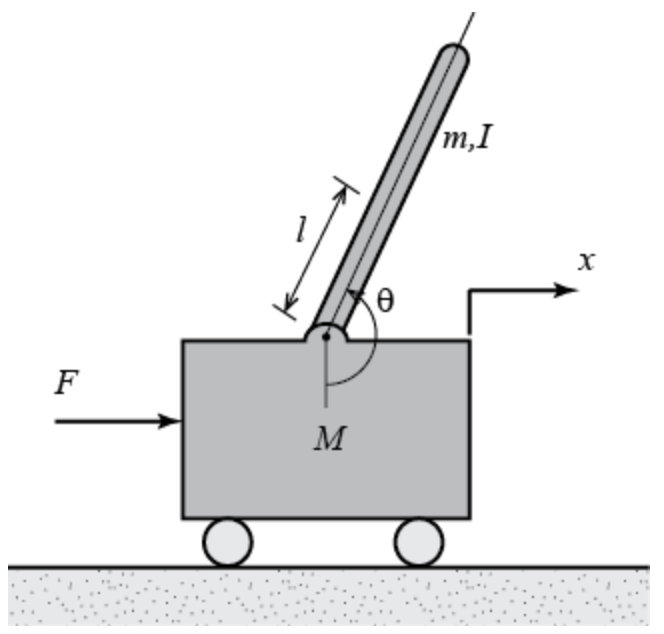
\includegraphics[width=.4\linewidth]{figures/pend.png}
    \caption{System Concept - Inverted Pendulum on a Cart \cite{inv}}
    \label{fig:pend}
\end{figure}

\subsubsection{Recording Constants}
\label{record}
In order to tune the gains of our system effectively, an accurate simulation model had to be created in MATLAB. For this to happen, all characteristics of the system, including the pendulum mass, inertia, cart mass, and more, had to be measured. In the case of cart friction, estimated.
\begin{figure}[H]
    \centering
    \begin{subfigure}{.49\textwidth}
      \centering
      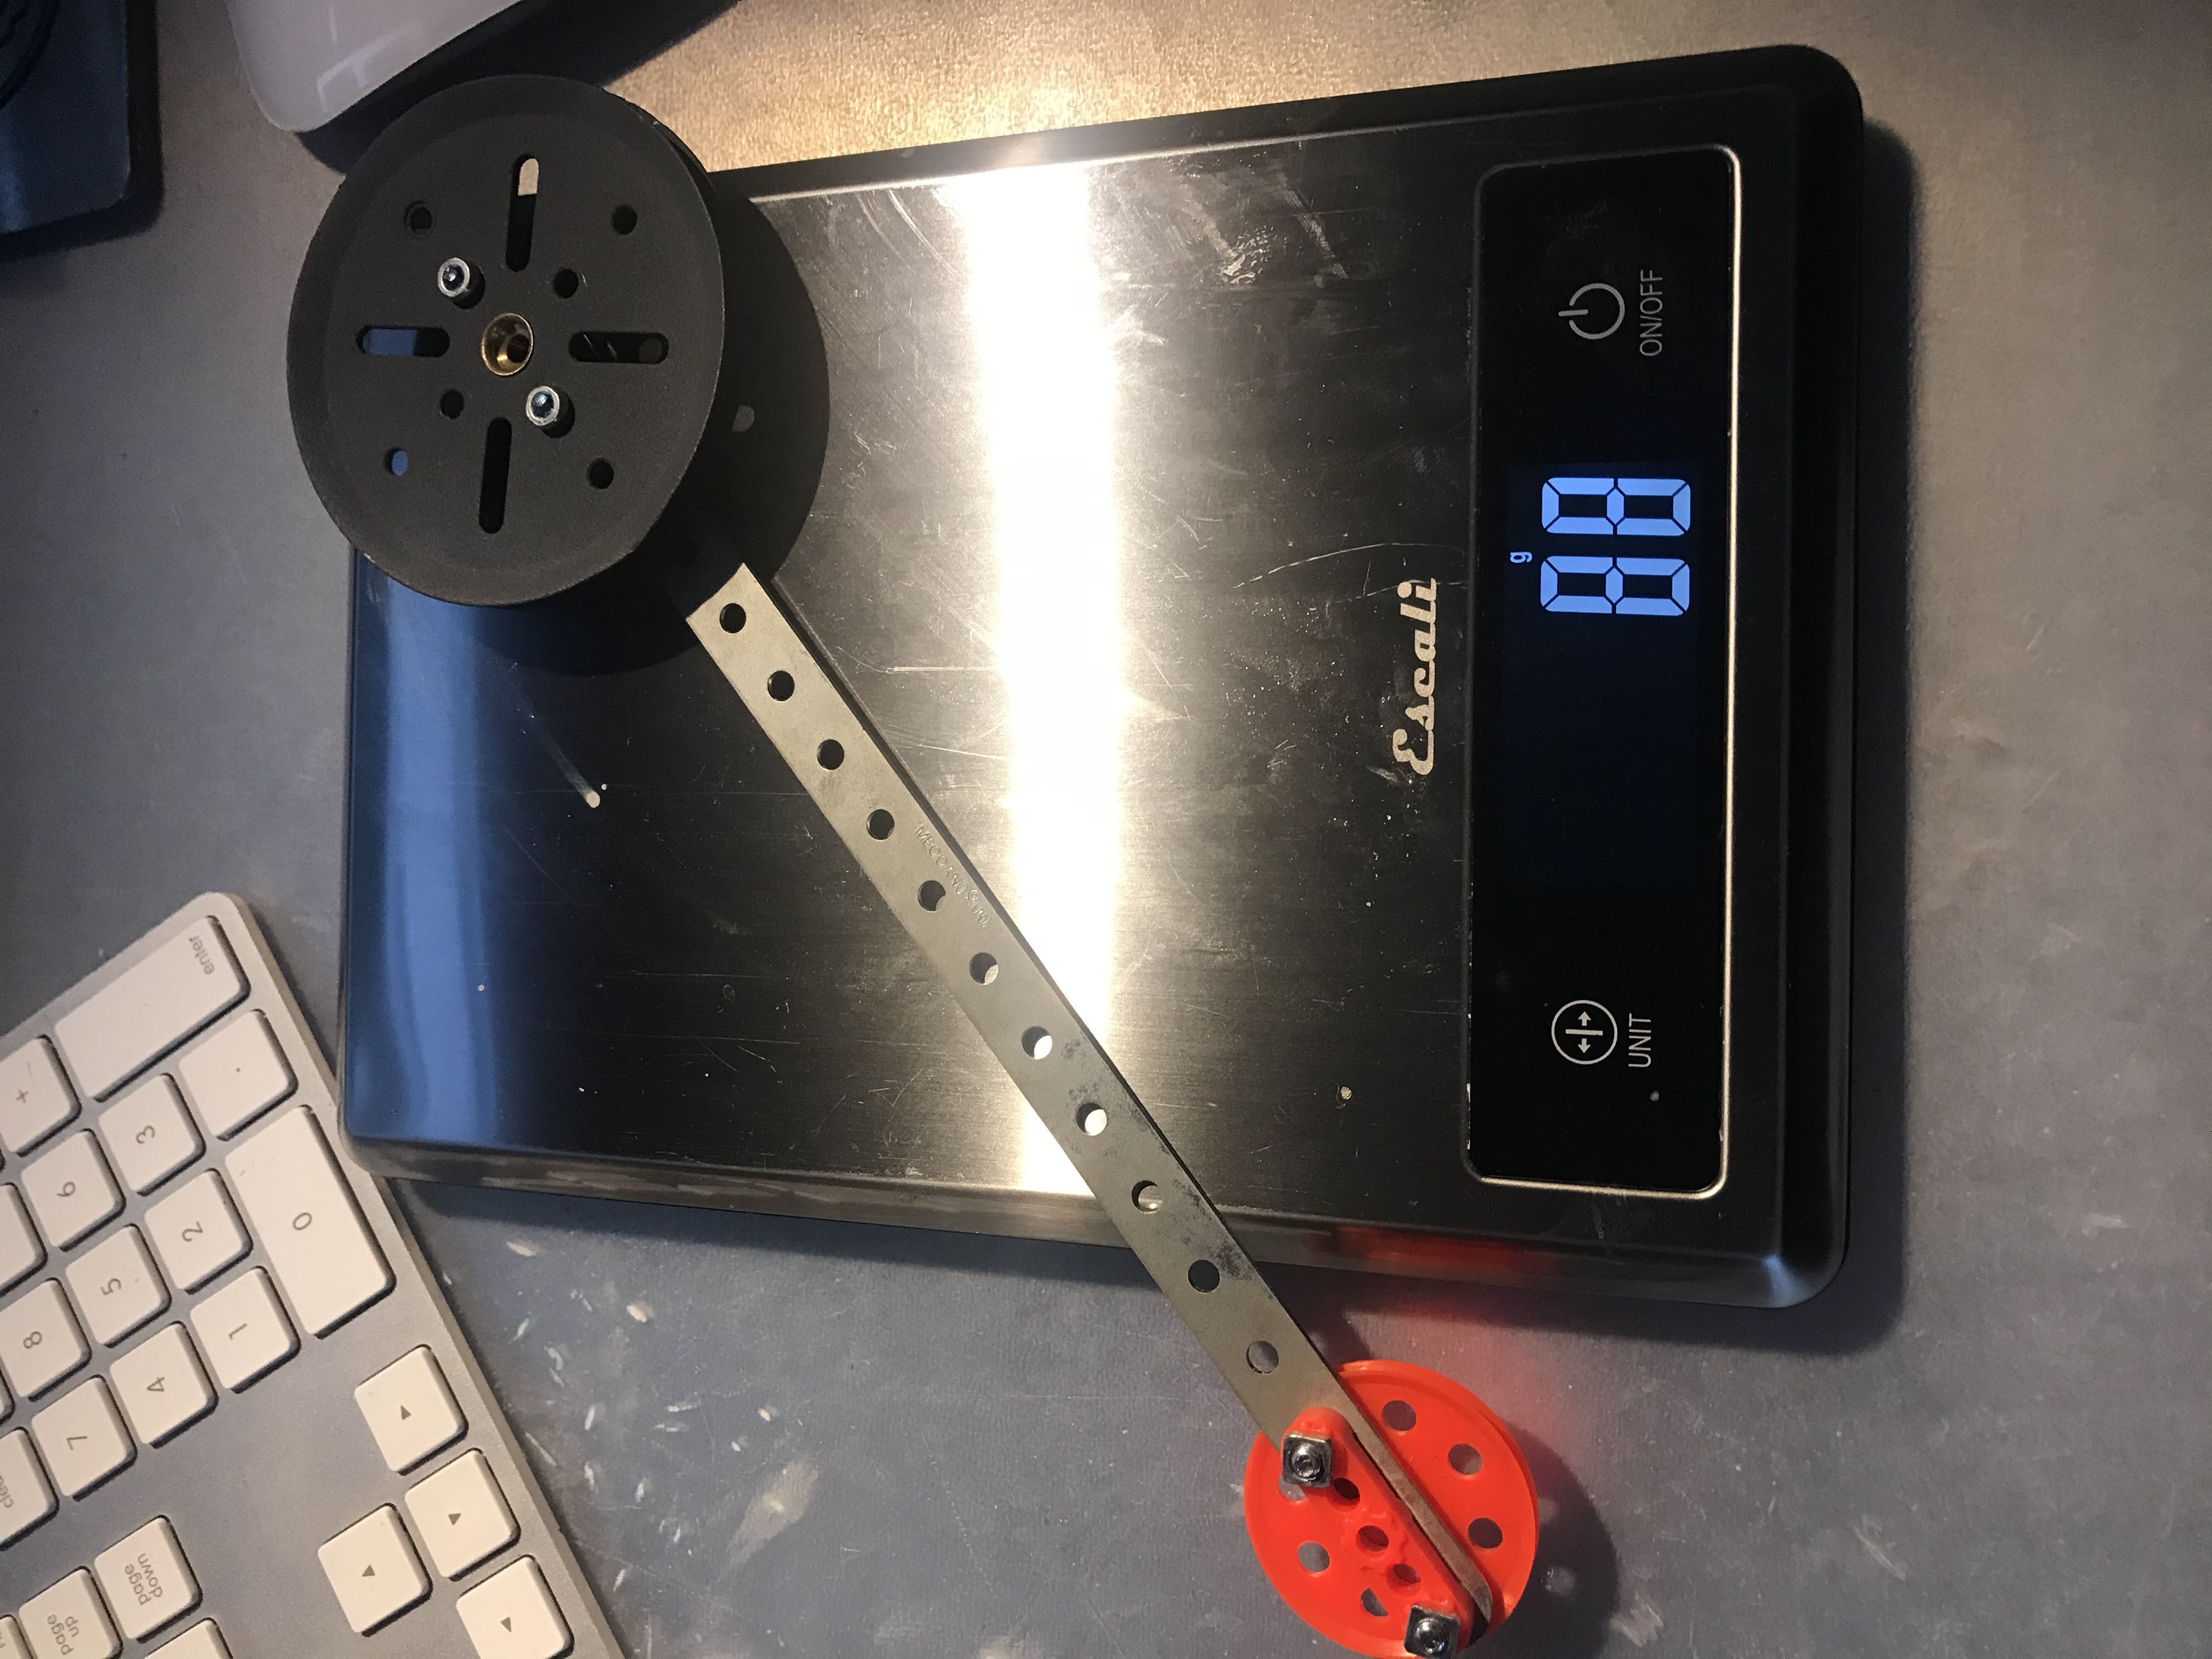
\includegraphics[width=1\linewidth]{figures/weigh1.jpg}
      \caption{Pendulum Mass}
      \label{fig:pMass}
    \end{subfigure}
    \begin{subfigure}{.49\textwidth}
      \centering
      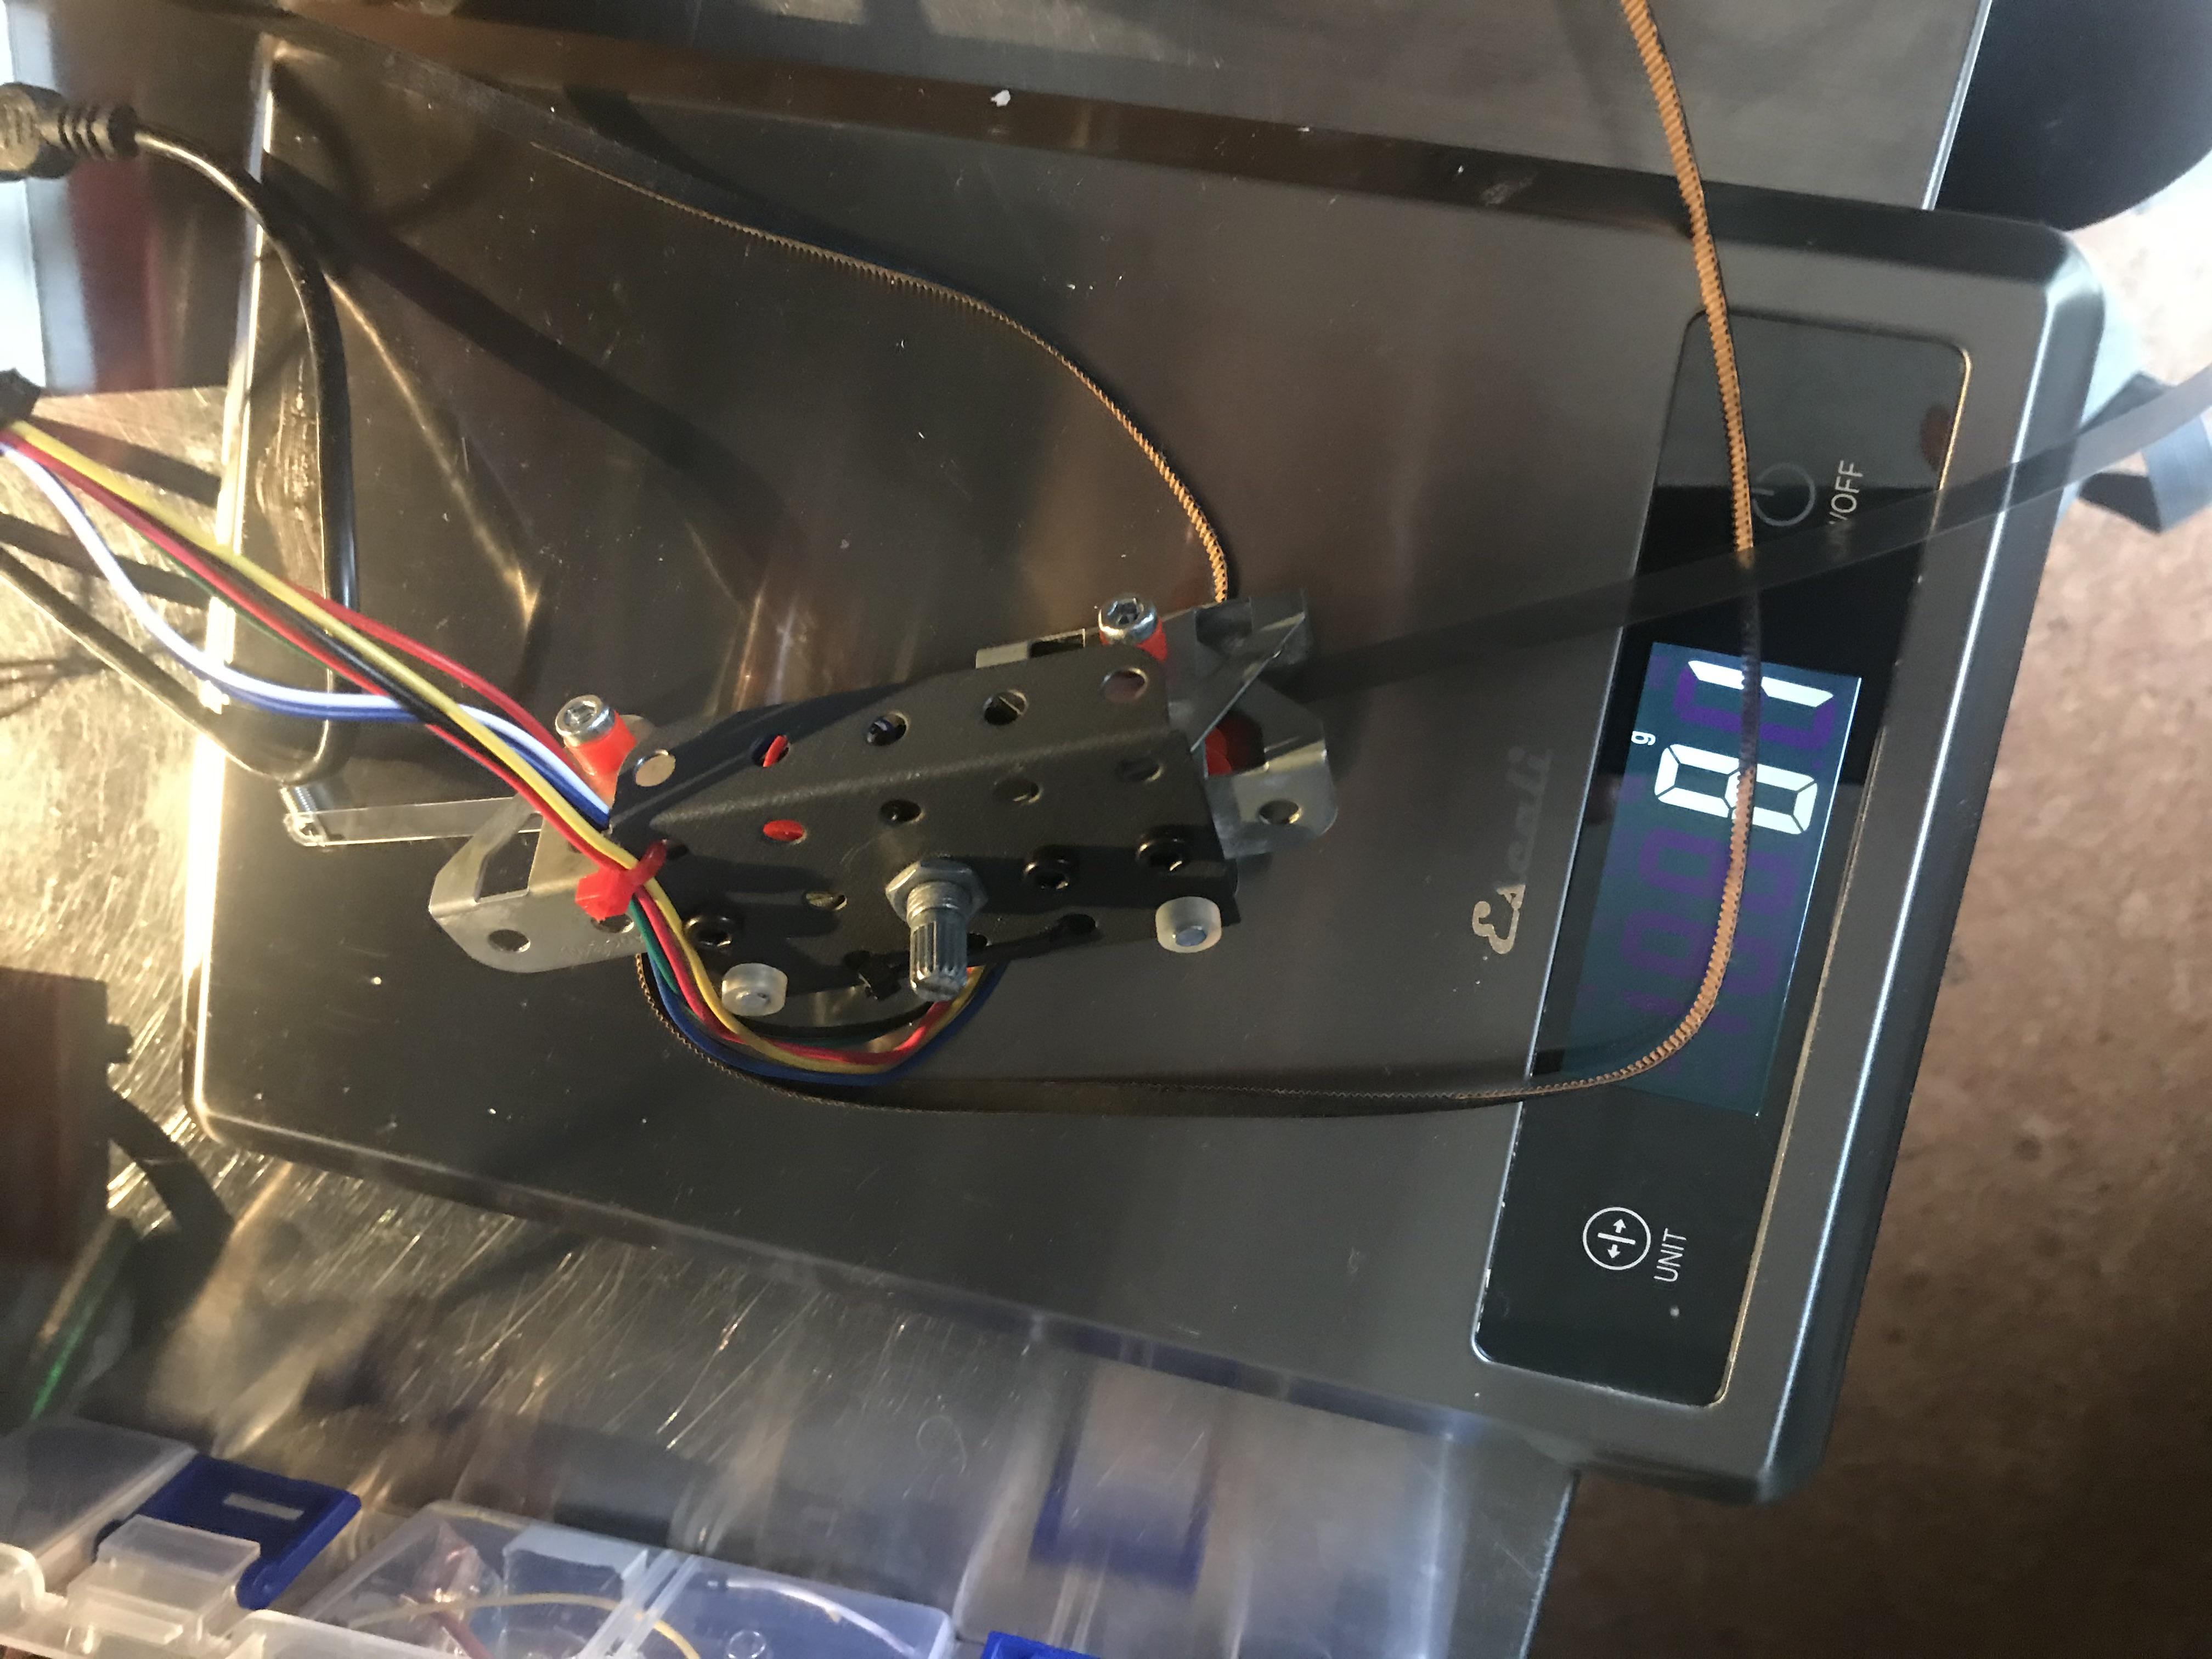
\includegraphics[width=1\linewidth]{figures/weigh2.jpg}
      \caption{Cart Mass}
      \label{fig:cMass}
    \end{subfigure}
    \caption{Measurement of System Constants}
    \label{fig:measure}
\end{figure}
All resulting MATLAB code can be seen in the \textit{model.m} file on Github \cite{github}. In order to make the derivation and linearization of the model, the variables for the model were defined as shown below: \\\\
\textbf{Model Variables}
\begin{itemize}
    \item $M$ mass of the cart = 0.081kg
    \item $m$ mass of the pendulum = 0.088kg 
    \item $b$ Cart friction estimate = 0.1N/m/s
    \item $g$ gravity coefficient = $9.81m/s^2$
    \item $l$ length of the pendulum = 0.10m
\end{itemize}
To add weight to the pendulum, a disk has been attached to the top. Without this weight, the pendulum is too light to overcome the static friction of the potentiometer, hence it remains in the same position unless the cart is moved repidly. In order to calculate the inertia of the pendulum, the following equation and variables were used.
\begin{itemize}
    \item $m_r_o_d$ mass of the rod = 0.035kg
    \item $m_d_i_s_k$ mass of the disk = 0.053kg 
    \item $r_d_i_s_k$ radius of the disk = 0.037m
\end{itemize}
\begin{equation}
   I = (1/3)*m_r_o_d*l^2 + 0.5*m_d_i_s_k*r_d_i_s-k^2 + m_d_i_s_k*(2*l + r_d_i_s_k)^2
\end{equation}


\subsection{Dynamic Equations}
After summing up all the forces acting on the cart and the pendulum in figure 4, the dynamic equation are shown below:
\begin{equation}
    (M+m)\ddot{x} + bx +ml\ddot{\theta}cos(\theta) - ml(\dot{\theta})^2sin(\theta) = F 
\end{equation}
\begin{equation}
    (I+ml^2)\ddot{\theta} + mglsin\theta = -ml\ddot{x}cos\theta
\end{equation}
\subsection{Linearization}
As the system to which the equations will be applied is linear, so the equations need to be linearized. The equations are linearized about vertical equilibrium position and assuming small deviation from the equilibrium position, small angle approximations were made for the nonlinear function for the system. 
\begin{equation}
    \theta{\approx}\pi, \phi = \pi - \phi
\end{equation}
\begin{equation}
    cos(\theta) = cos(\pi + \phi){\approx} -1
\end{equation}
\begin{equation}
    sin(\theta) = sin(\pi + \phi){\approx} -\phi
\end{equation}
\begin{equation}
    \dot{\theta} = \dot{\phi}{\approx} 0
\end{equation}
The equation for the model after linearization is shown below
\begin{equation}
    (M+m)\ddot{x} + bx +ml\ddot{\theta} = u
\end{equation}
\begin{equation}
    (I+ml^2)\ddot{\theta} + mgl\theta = -ml\ddot{x}
\end{equation}
\subsection{Resulting State Space Model}
\begin{center}
    \begin{bmatrix}
    \dot{x}\\
    \ddot{x}\\
    \dot{\theta}\\
    \ddot{\theta}
    \end{bmatrix}
    =
    \begin{bmatrix}
    0 & 1 & 0 & 0\\
    0 & -(I+ml^2)b/p & m^2gl^2/p & 0\\
    0 & 0 & 0 & 1\\
    0 & -(mlb)/p & mgl(M+m)/p & 0
    \end{bmatrix}
    \begin{bmatrix}
    x\\
    \dot{x}\\
    \theta\\
    \dot{\theta}
    \end{bmatrix}
    +
    \begin{bmatrix}
    0\\
    (I+ml^2)/p\\
    0\\
    ml/p
    \end{bmatrix}
    u
\end{center}
\begin{center}
    

    y = 
    \begin{bmatrix}
    1 & 0 & 0 & 0\\
    0 & 0 & 1 & 0
    \end{bmatrix}
    \begin{bmatrix}
    x\\
    \dot{x}\\
    \theta\\
    \dot{\theta}
    \end{bmatrix}
    +
    \begin{bmatrix}
    0\\
    0
    \end{bmatrix}
    u \\
    \begin{equation}
   \textrm{Where } p = I*(M+m) + M*m*l^2 %denominator for the A and B matrices
\end{equation}
\end{center}
The variables value for our model were plugged into the state space and the resultant matrix is shown below\\\\
\begin{center}
    

\begin{bmatrix}
\dot{x}\\
\ddot{x}\\
\dot{\theta}\\
\ddot{\theta}
\end{bmatrix}
=
\begin{bmatrix}
0 & 1 & 0 & 0\\
0 & -0.6681 & 1.2657 & 0\\
0 & 0 & 0 & 1\\
0 & -1.4661 & 24.31 & 0
\end{bmatrix}
\begin{bmatrix}
x\\
\dot{x}\\
\theta\\
\dot{\theta}
\end{bmatrix}
+
\begin{bmatrix}
0\\
5.215\\
0\\
14.66
\end{bmatrix}
u \\\\
y = 
\begin{bmatrix}
1 & 0 & 0 & 0\\
0 & 0 & 1 & 0
\end{bmatrix}
\begin{bmatrix}
x\\
\dot{x}\\
\theta\\
\dot{\theta}
\end{bmatrix}
+
\begin{bmatrix}
0\\
0
\end{bmatrix}
u \\\\
\end{center}
\subsubsection{Controllability}
Controllability is the ability of the controller to randomly change the function of the system. To calculate controllability the equation used is shown below\\
\begin{equation}
    P = [B \;AB\; ......\; A^{n-1}B]
\end{equation}
The controllability of the system was checked in MATLAB with the formula \textbf{ctrb}(A,B), resulting in a value of 4, implying that \textit{P} is full rank, and thus the system is controllable.
\subsubsection{Observability}
Observability is the ability of the system to decide if the state variable of the system can be measured from the external outputs. To calculate the the observability the equation used is shown below\\
\begin{equation}
    Q = 
    \begin{bmatrix}
C\\
CA\\
.\\
.\\
CA^{n-1}
    \end{bmatrix}
\end{equation}
The observability of the system was checked in MATLAB with the formula \textbf{obsv}(C,A), resulting in a value of 4, implying the system is also observable.
\section{System Design}
\subsection{Requirements}
The requirements for this problem are short and sweet - to balance the pendulum vertically as opposed to letting it fall over due to gravity. To elaborate on these requirements, we can set the following parameters:
\begin{itemize}
    \item $\Delta \theta < 5^o$ for small impulses to the pendulum or cart.
    \item Settling time of $< 4$ seconds.
    \item Cart position should be settled consistently at a constant reference location, ie. $x=0cm$.
\end{itemize}
Further requirements may be set for the \textit{Nice to Have's} outlined in section \ref{nice}, depending on the project's completion schedule. Assuming all prior requirements are complete, we will investigate said problems and construct design requirements. 
\subsubsection{Nice to Have's}
\label{nice}
In addition the the objectives outline in the previous section, there are many sub-features that can be developed in the software of this system that present complex control theory problems, 2 of which are outlined below.
\begin{itemize}
    \item Side-stepping of cart to a desired position ensuring constant pendulum stability.\\ \indent - For example, move cart from $x=0cm$ to $x=10cm$ with minimal overshoot, rise time, steady state error.
    \item Swing-up and swing-down commands\\ \indent - Enables the system to move the cart from one state of stability to another, ie. from $\theta =0^o$ to $\theta =180^o$ and stabilize, or vice versa with minimum oscillation.
\end{itemize}
\subsection{State Feedback Control Model}
\label{theory}
The following control model will be implemented assuming full state feedback.
\begin{figure}[H]
    \centering
    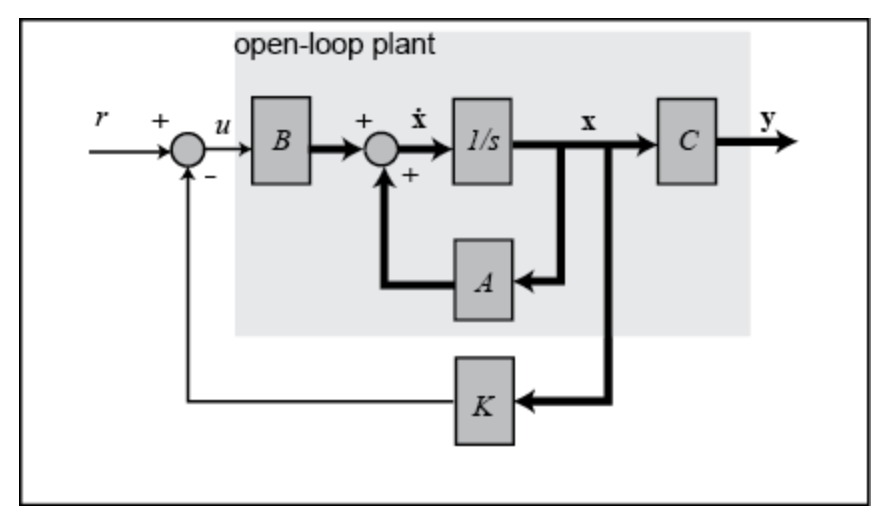
\includegraphics[width=.5\linewidth]{figures/fsfFlow.png}
    \caption{Full State Feedback Control Model  \cite{inv2}}
    \label{fig:fsf}
\end{figure}
The following equation represents the controller output \textit{u}, which effectively sets the duty cycle of the motor PWM signal, can be seen below.
\begin{equation}
    u = -Kx + r
\end{equation}
Where the values of K will be tuned in MATLAB. In order to model our system accurately in MATLAB, each constant of the system must be measured and recorded (see section \ref{record}). For example, the cart weight, pendulum inertia, length and more have significant impacts on the modelling of the system, including the controllability and observability. Once these values are recorded, MATLAB will also be used to tune the gain vector \textit{L}, also known as the Luenberger observer, based off the closed loop system poles.
\subsubsection{Linear Quadratic Regulator Control}
Following the initial implementation of this control system, a more enhanced linear quadratic regulator controller will be implemented. This system, though similar in practicality to a PID controller, employs a more optimal approach to gain tuning. Essentially, gains  "are found by using a mathematical algorithm that minimizes a cost function with weighting factors supplied by a human (engineer)" \cite{lqr}. Said function to minimize, for a finite horizon discrete time system, is shown below.
\begin{equation}
    \centering
    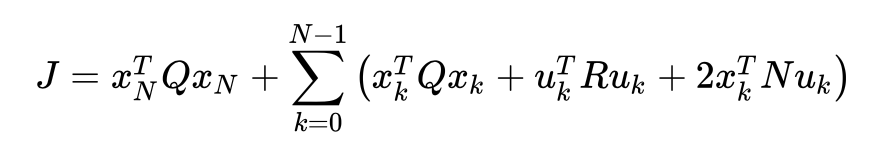
\includegraphics[width=.6\linewidth]{figures/lqr.png}
\end{equation}
The performance index \textit{J} is to be minimized. By tuning values in Q and the value of R, the gains and closed loop system poles are optimized according to these requirements. To achieve this function in MATLAB, the \textbf{dlqr} command will be used for implementation with a discrete time system.
\subsubsection{Luenberger Observer}
Physical systems possess many non-linearities and thus more practical models and tuning will need to be implemented. Such as the problem of the nonlinear control of an inverted pendulum, which sees to balance the pendulum from an unstable equilibrium position. Such control methods include Linear Quadratic Regulation (LQR), observer based state feedback control and more. The following flowchart displays the proposed observer based state feedback control model, implementing an observer due to the fact that the system does not provide full state feedback, which would require the purchase of 2 tachometers to measure the rate of change of $\theta, x$, that is, $\dot{\theta}, \dot{x}$. However, we will be implementing a state estimator to estimate the values of these states instead.
\begin{figure}[H]
    \centering
    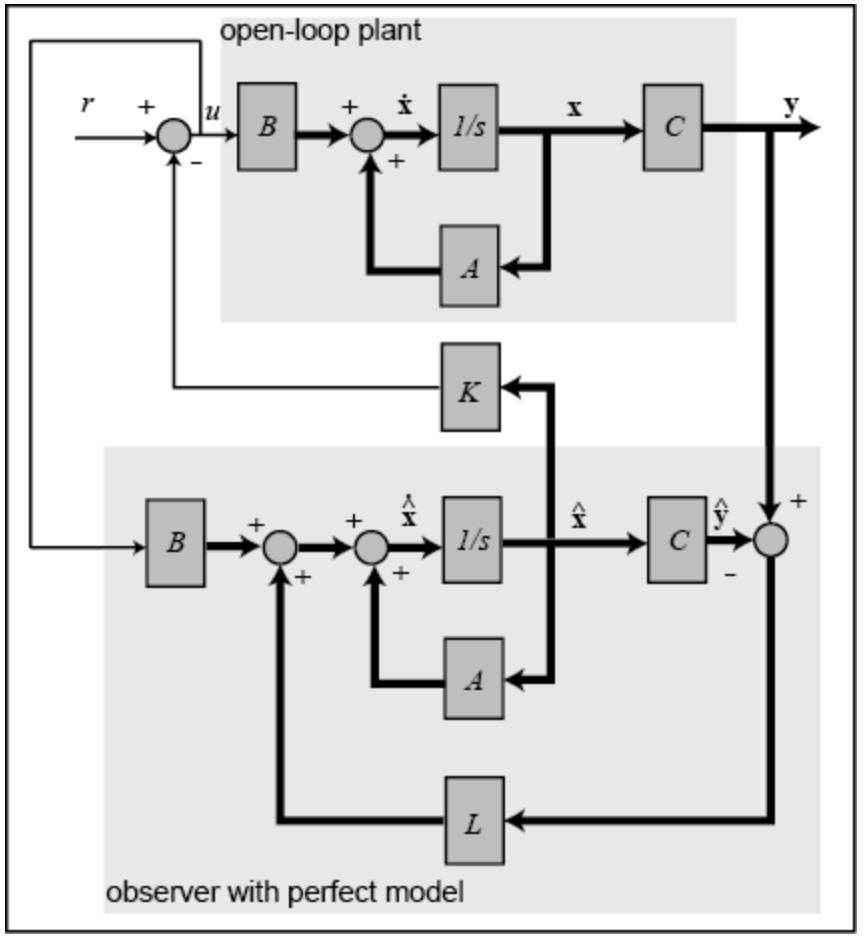
\includegraphics[width=.5\linewidth]{figures/flow.png}
    \caption{Observer Based State Feedback Model \cite{inv2}}
    \label{fig:fc}
\end{figure}
The above control system will not be elaborated too in depth as it is out of the scope of this report, however it presents the overall concept. The most important variables and what they represent are discussed in the following:
\begin{itemize}
    \item $x$ the states of the system - $x, \dot{x}, \theta, \dot{\theta}$, measured and estimated through observer based state feedback.
    \item $y$ the demanded outputs of the controller, $x, \theta$
    \item $u$ the inputs to the system, which would be the force to the cart, $F$.
    \item $K, L$, the gain vector and Luenberger observer vector, designed and tuned in MATLAB.
    \item All other matrices, $A, B, C, D$ and so forth, represent the complete state model for the linearized system, full form shown below:
\end{itemize}
\begin{equation}
    \dot{x} = Ax + Bu \textrm{ and }
    y = Cx + Du
\end{equation}
And for the state estimator:
\begin{equation}
    \dot{\hat{x}} = A\hat{x} + Bu + L(y-\hat{y}) \textrm{ and }
    \dot{e} = \dot{x} - \dot{\hat{x}} = ... \implies \dot{e} = (A - LC)e
    \label{eq}
\end{equation}
Who's poles will be designed as 5-10 times faster than that of the LQR controller, so as to drive \textbf{$e\implies0$} quickly and in a stable manner.

\section{Implementation}
\subsection{Hardware}
\subsubsection{Mechanical}
As for the hardware of the inverted pendulum system, the re-purposed Canon printer can be seen throughout the following figures.

\begin{figure}[H]
\centering
\begin{subfigure}{.5\textwidth}
  \centering
  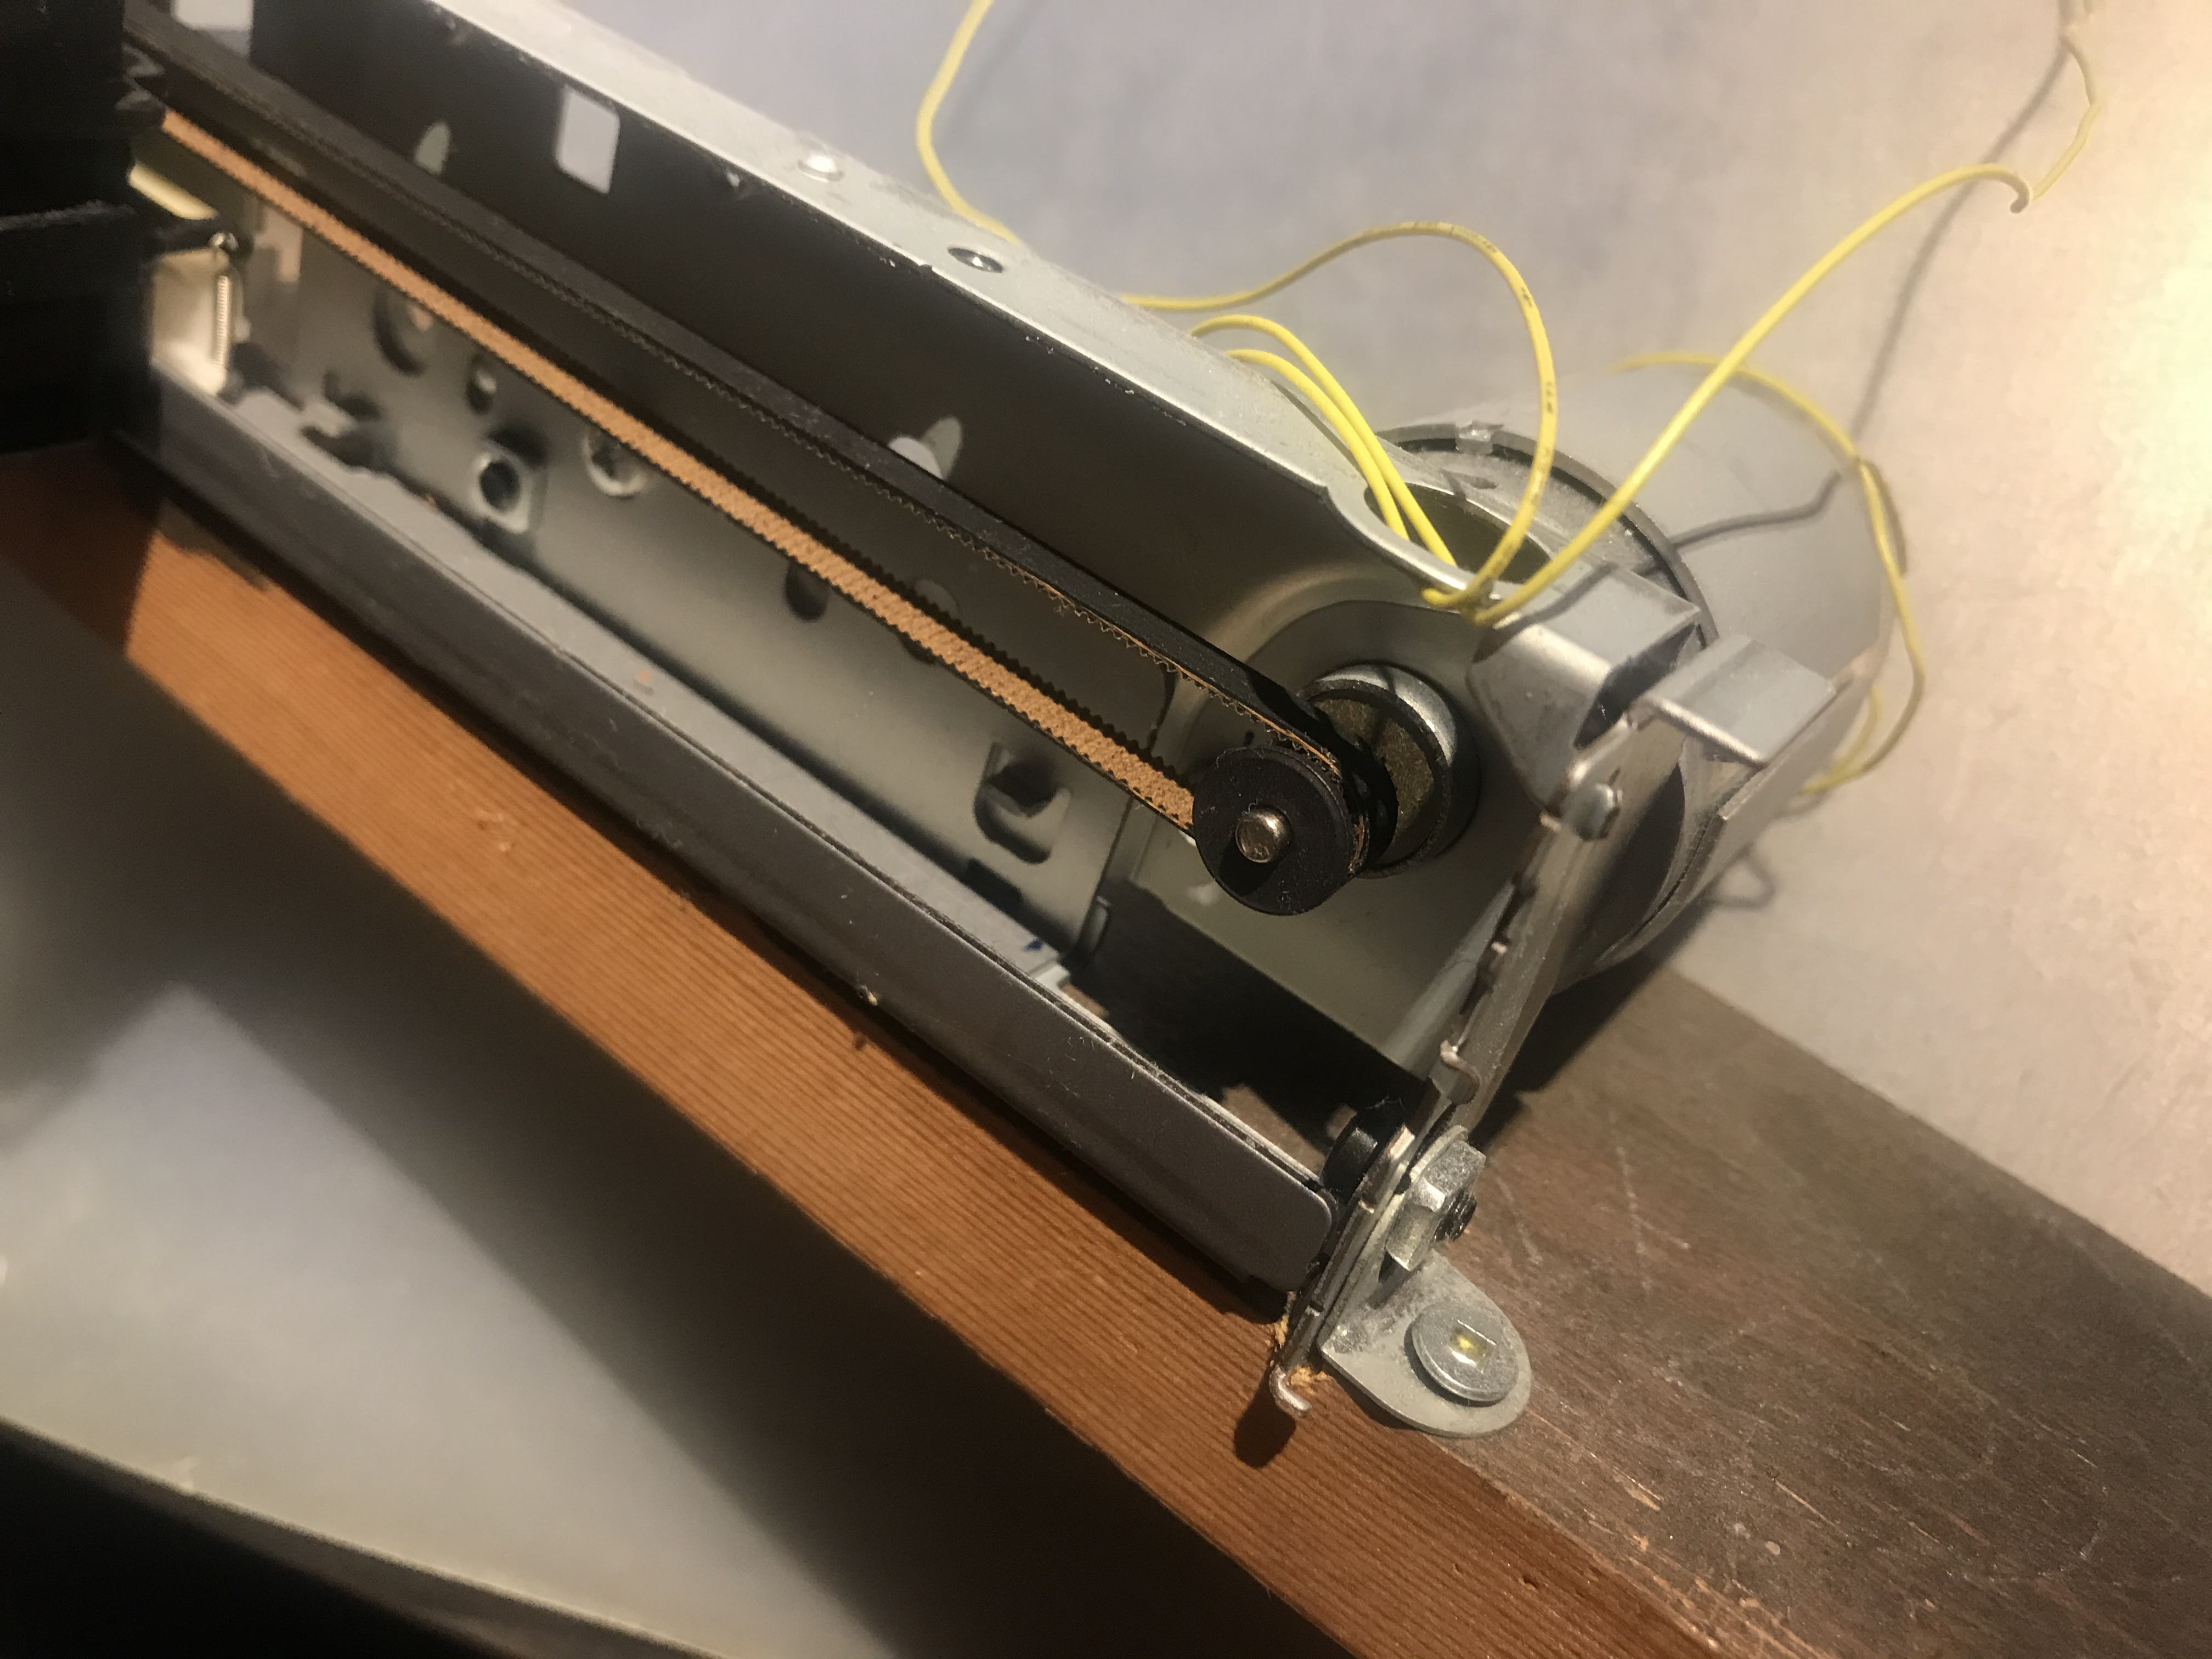
\includegraphics[width=1\linewidth]{figures/IMG_5674.jpg}
  \caption{DC Motor Belt Drive}
  \label{fig:dc}
\end{subfigure}%
\begin{subfigure}{.5\textwidth}
  \centering
  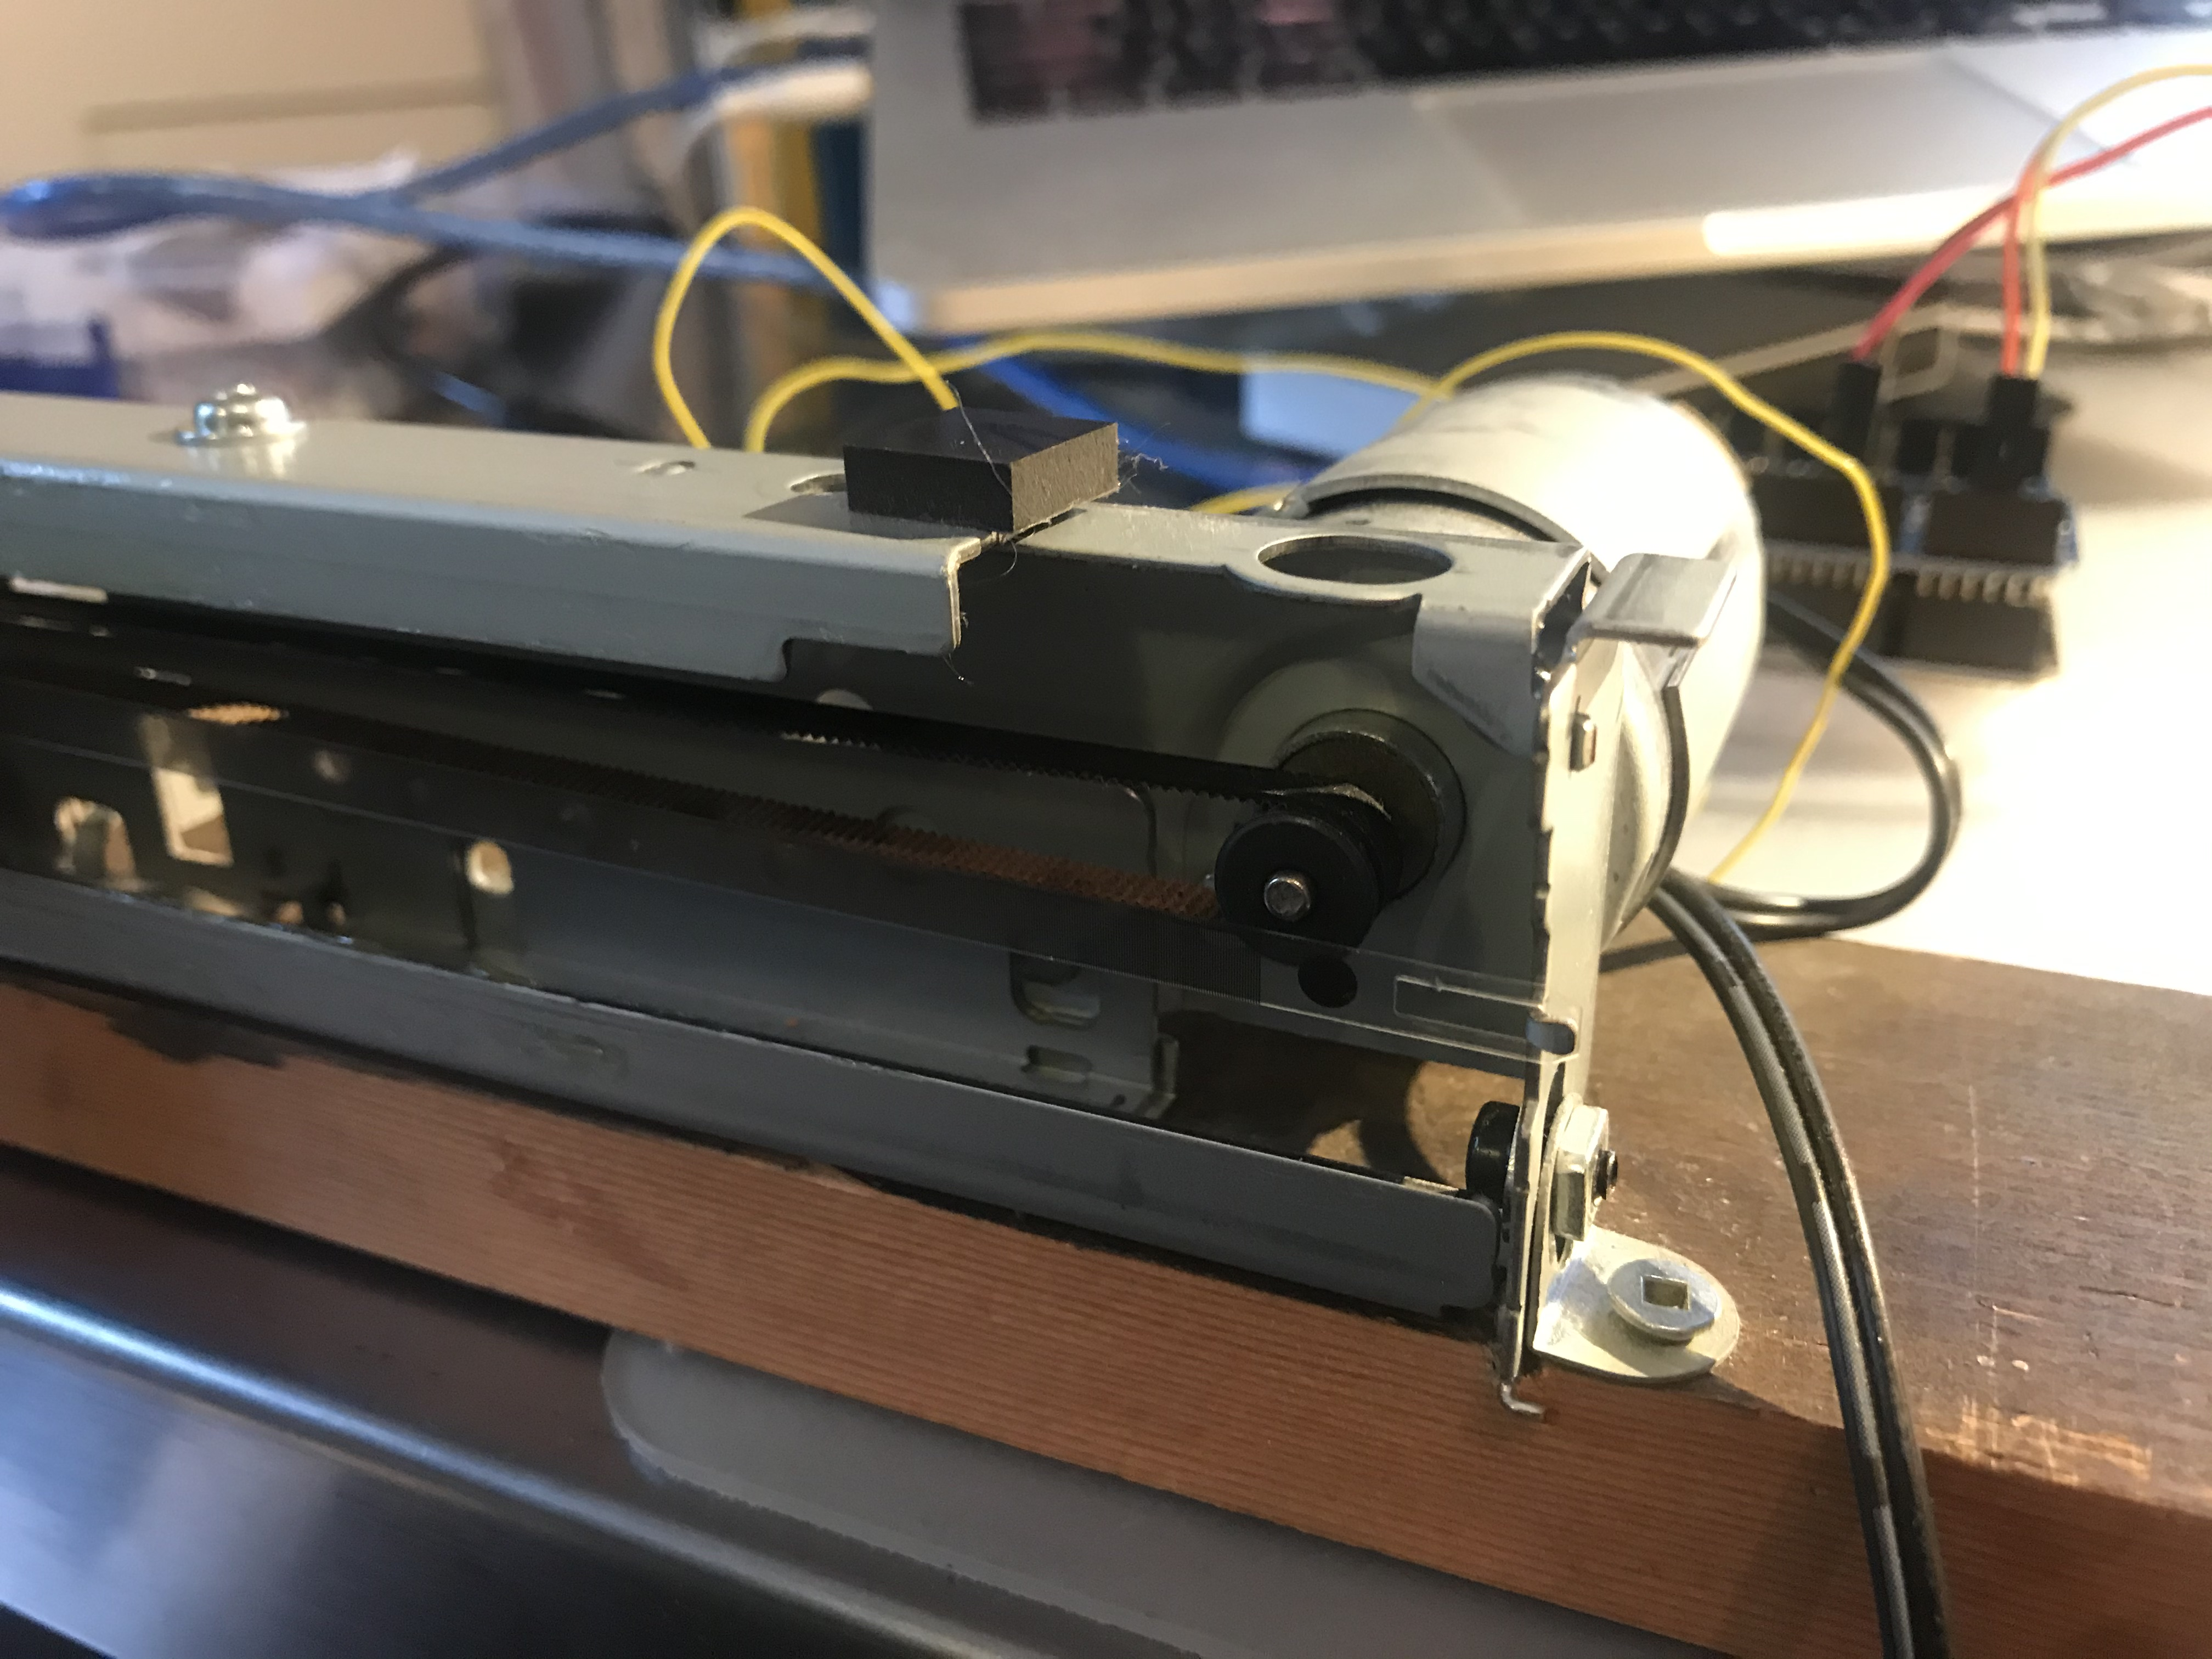
\includegraphics[width=1\linewidth]{figures/IMG_5807.jpg}
  \caption{Optical Encoder Linear Strip}
  \label{fig:opt}
\end{subfigure}
\caption{DC Motor Belt and Feedback}
\end{figure}

\begin{figure}[H]
\centering
\begin{subfigure}{.5\textwidth}
  \centering
  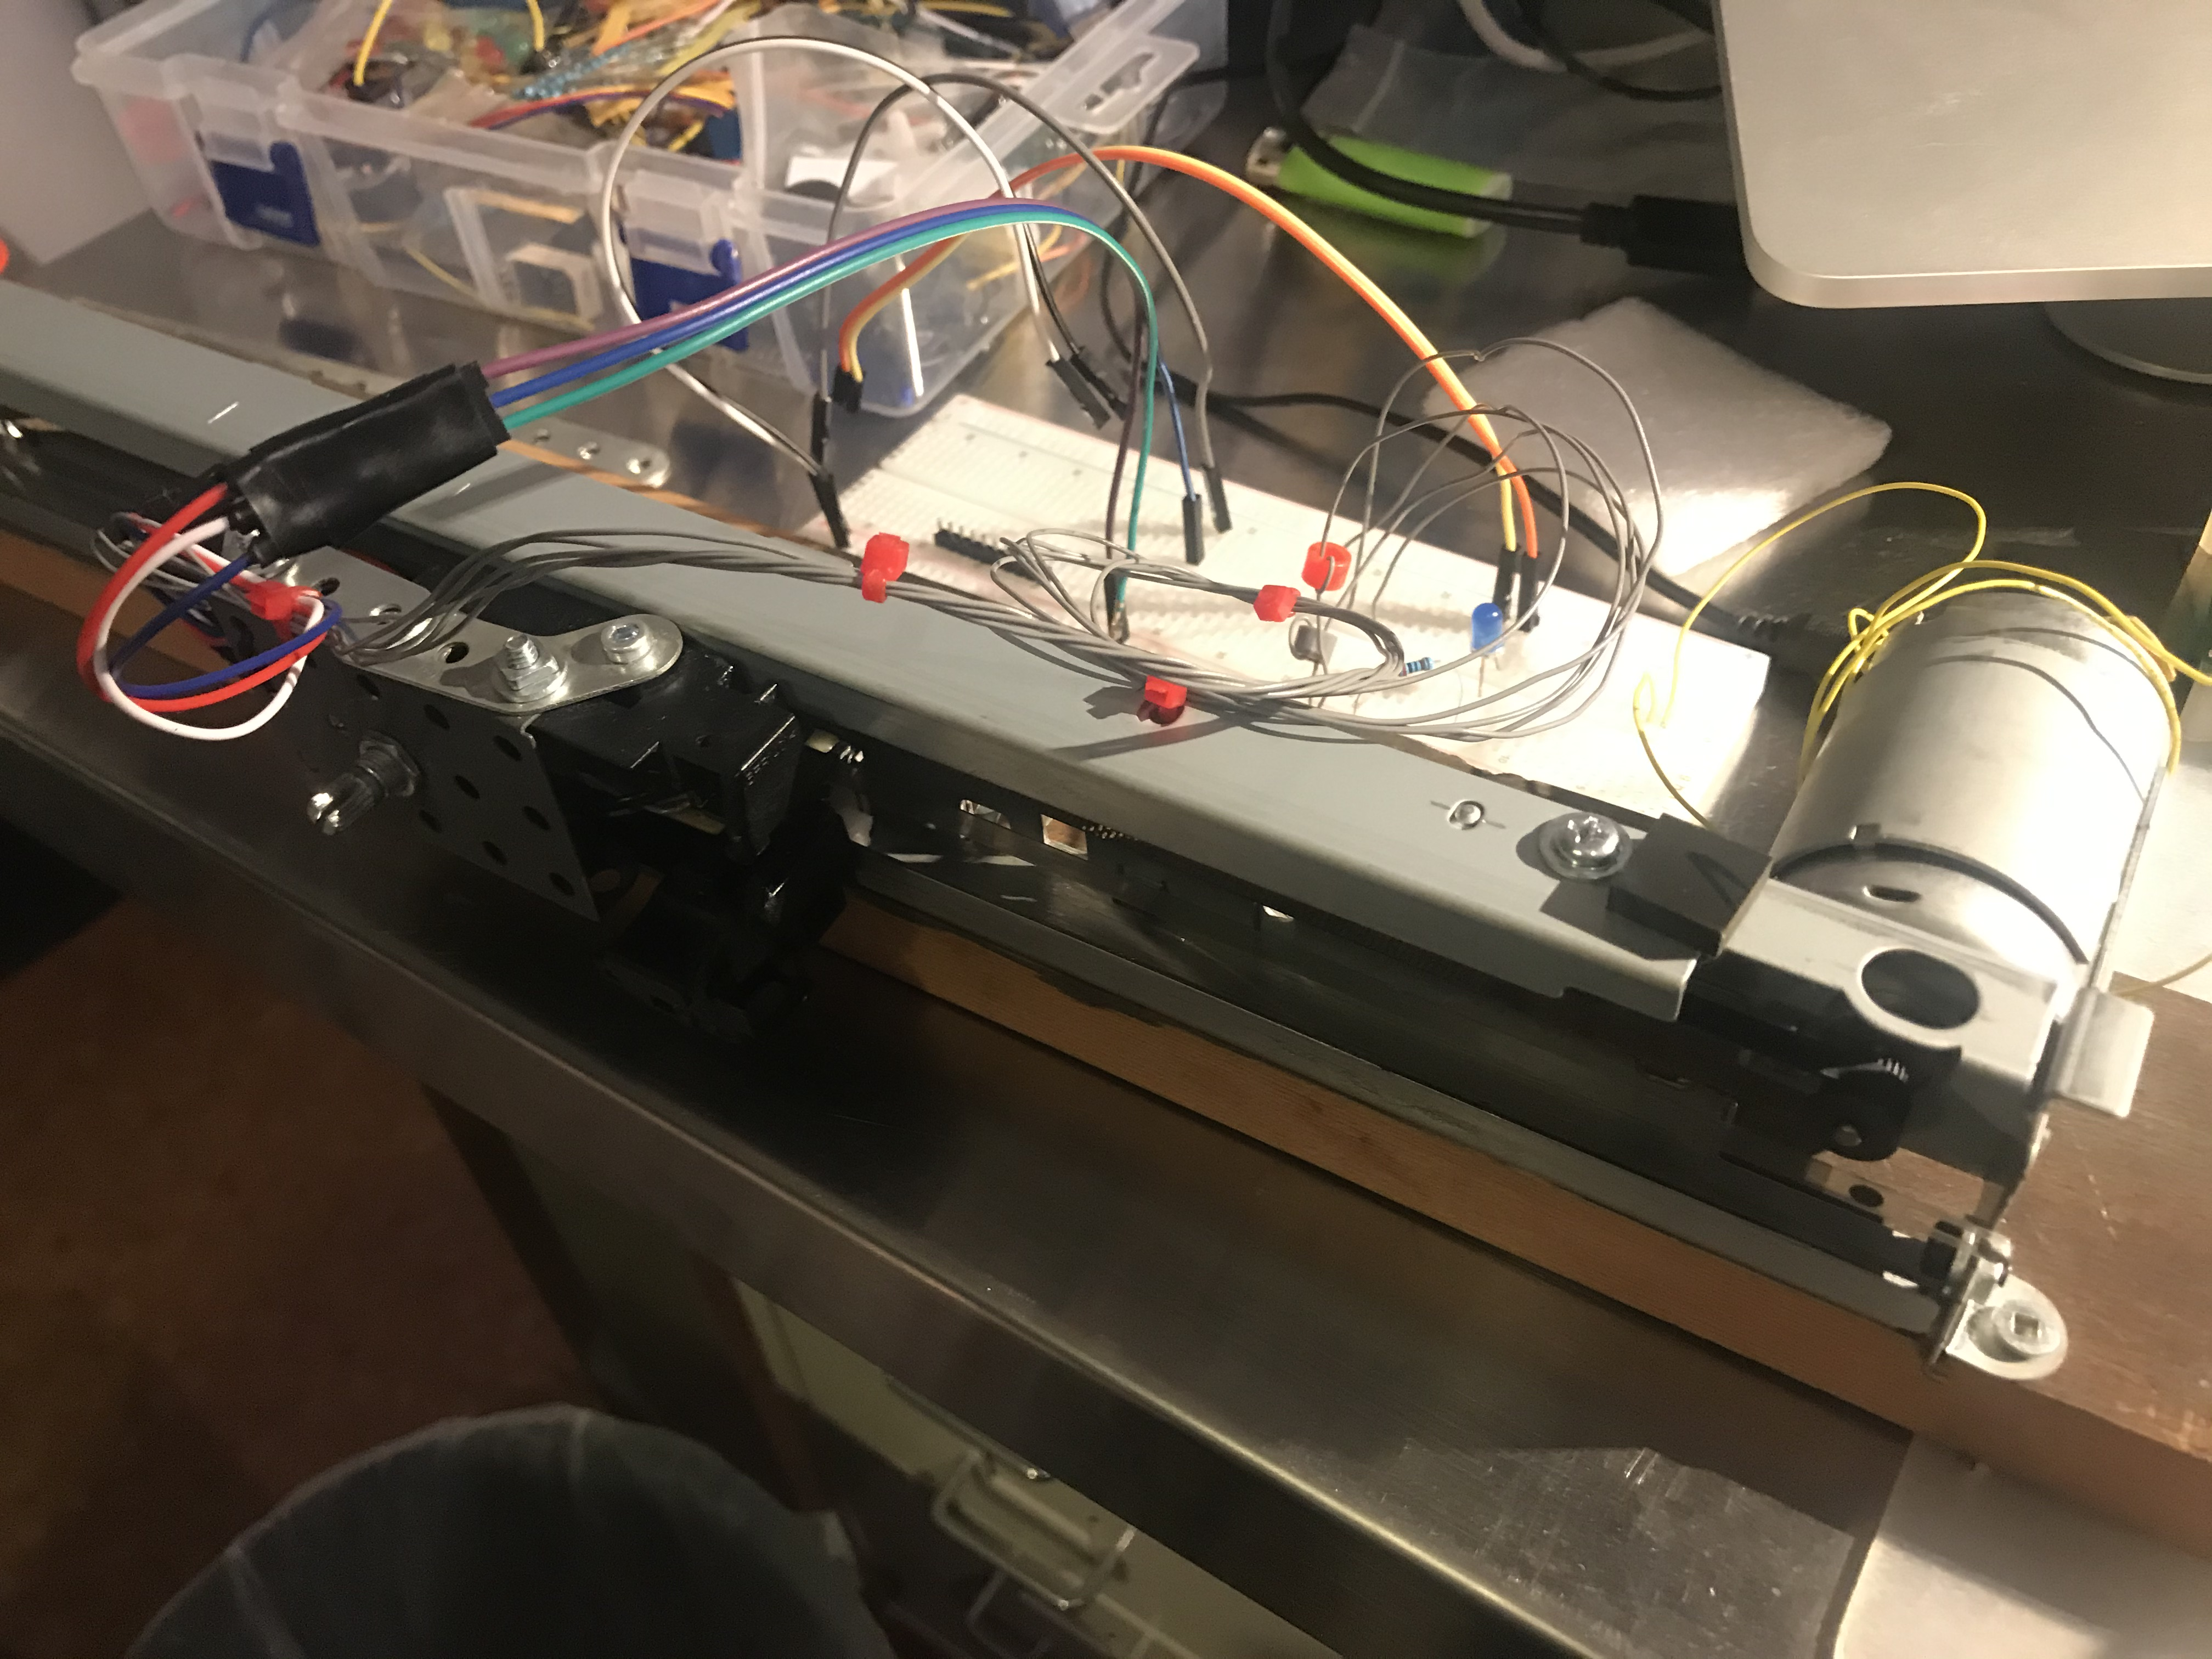
\includegraphics[width=1\linewidth]{figures/IMG_5831.jpg}
    \caption{System Setup with Wiring}
    \label{fig:wire}
\end{subfigure}%
\begin{subfigure}{.5\textwidth}
  \centering
  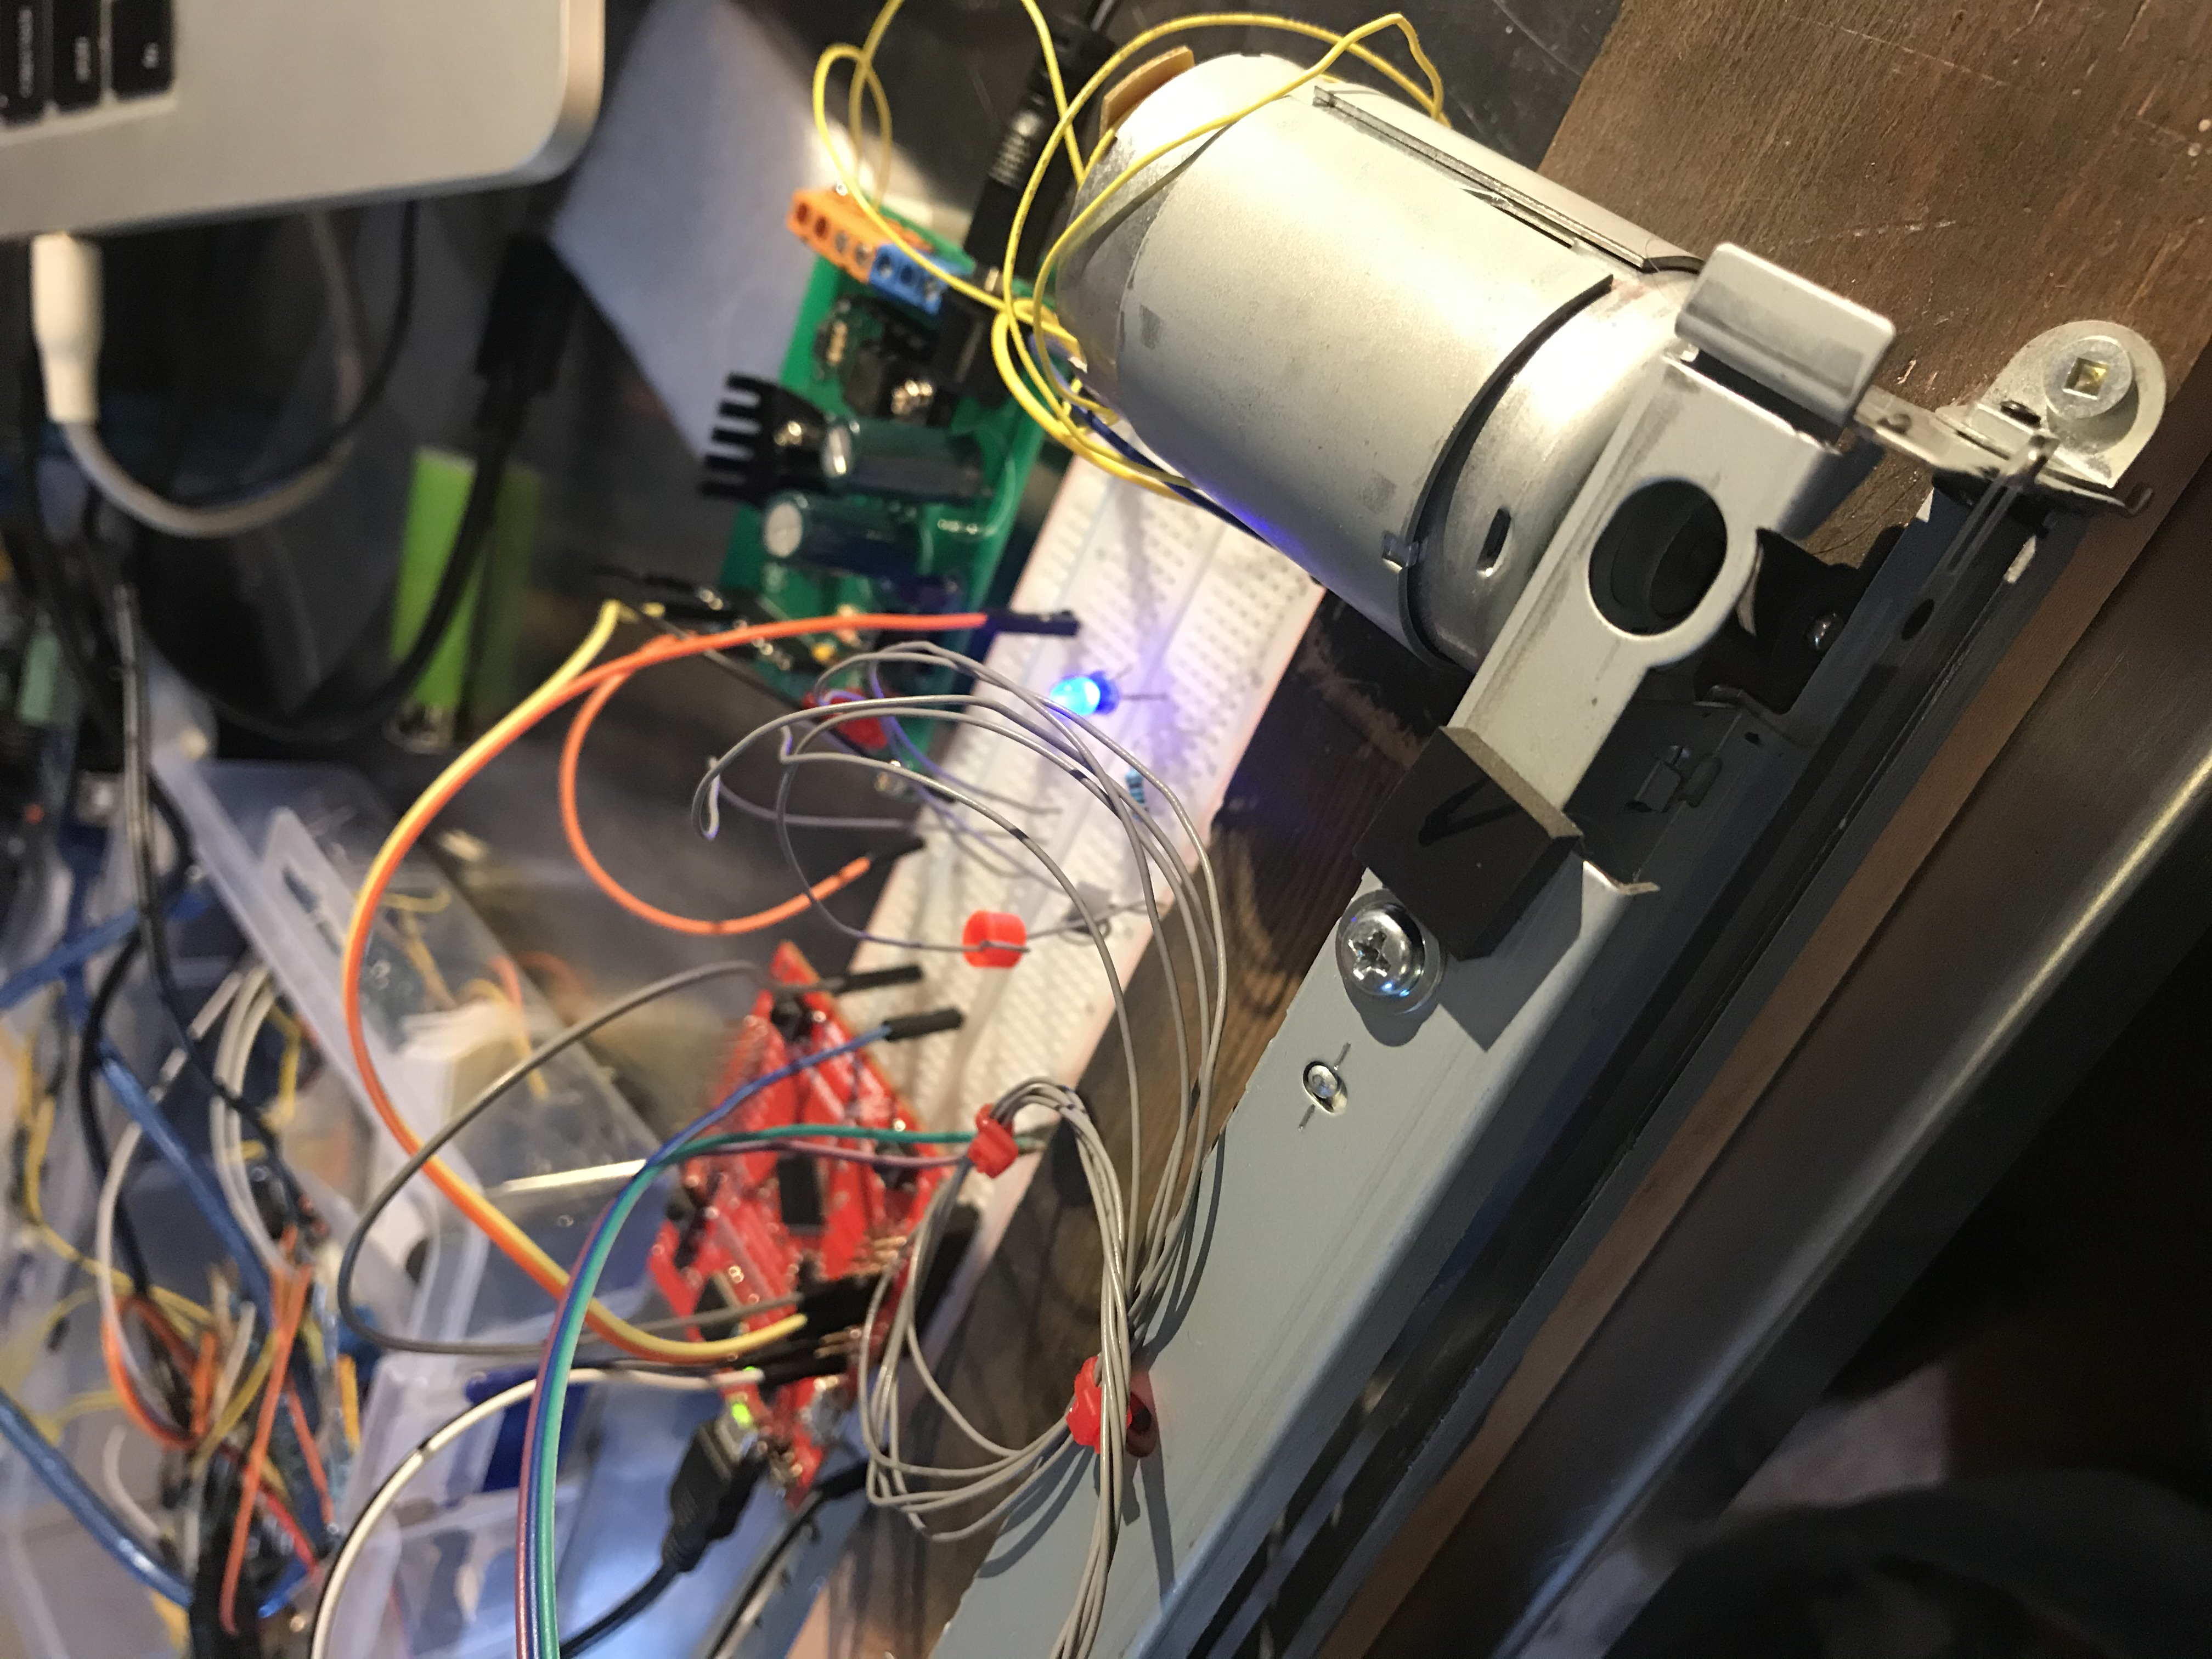
\includegraphics[width=1\linewidth]{figures/IMG_5848.jpg}
    \caption{System Electronics}
    \label{fig:elec}
\end{subfigure}
\caption{System Setup Development}
\end{figure}

\begin{figure}[H]
\centering
\begin{subfigure}{.5\textwidth}
  \centering
  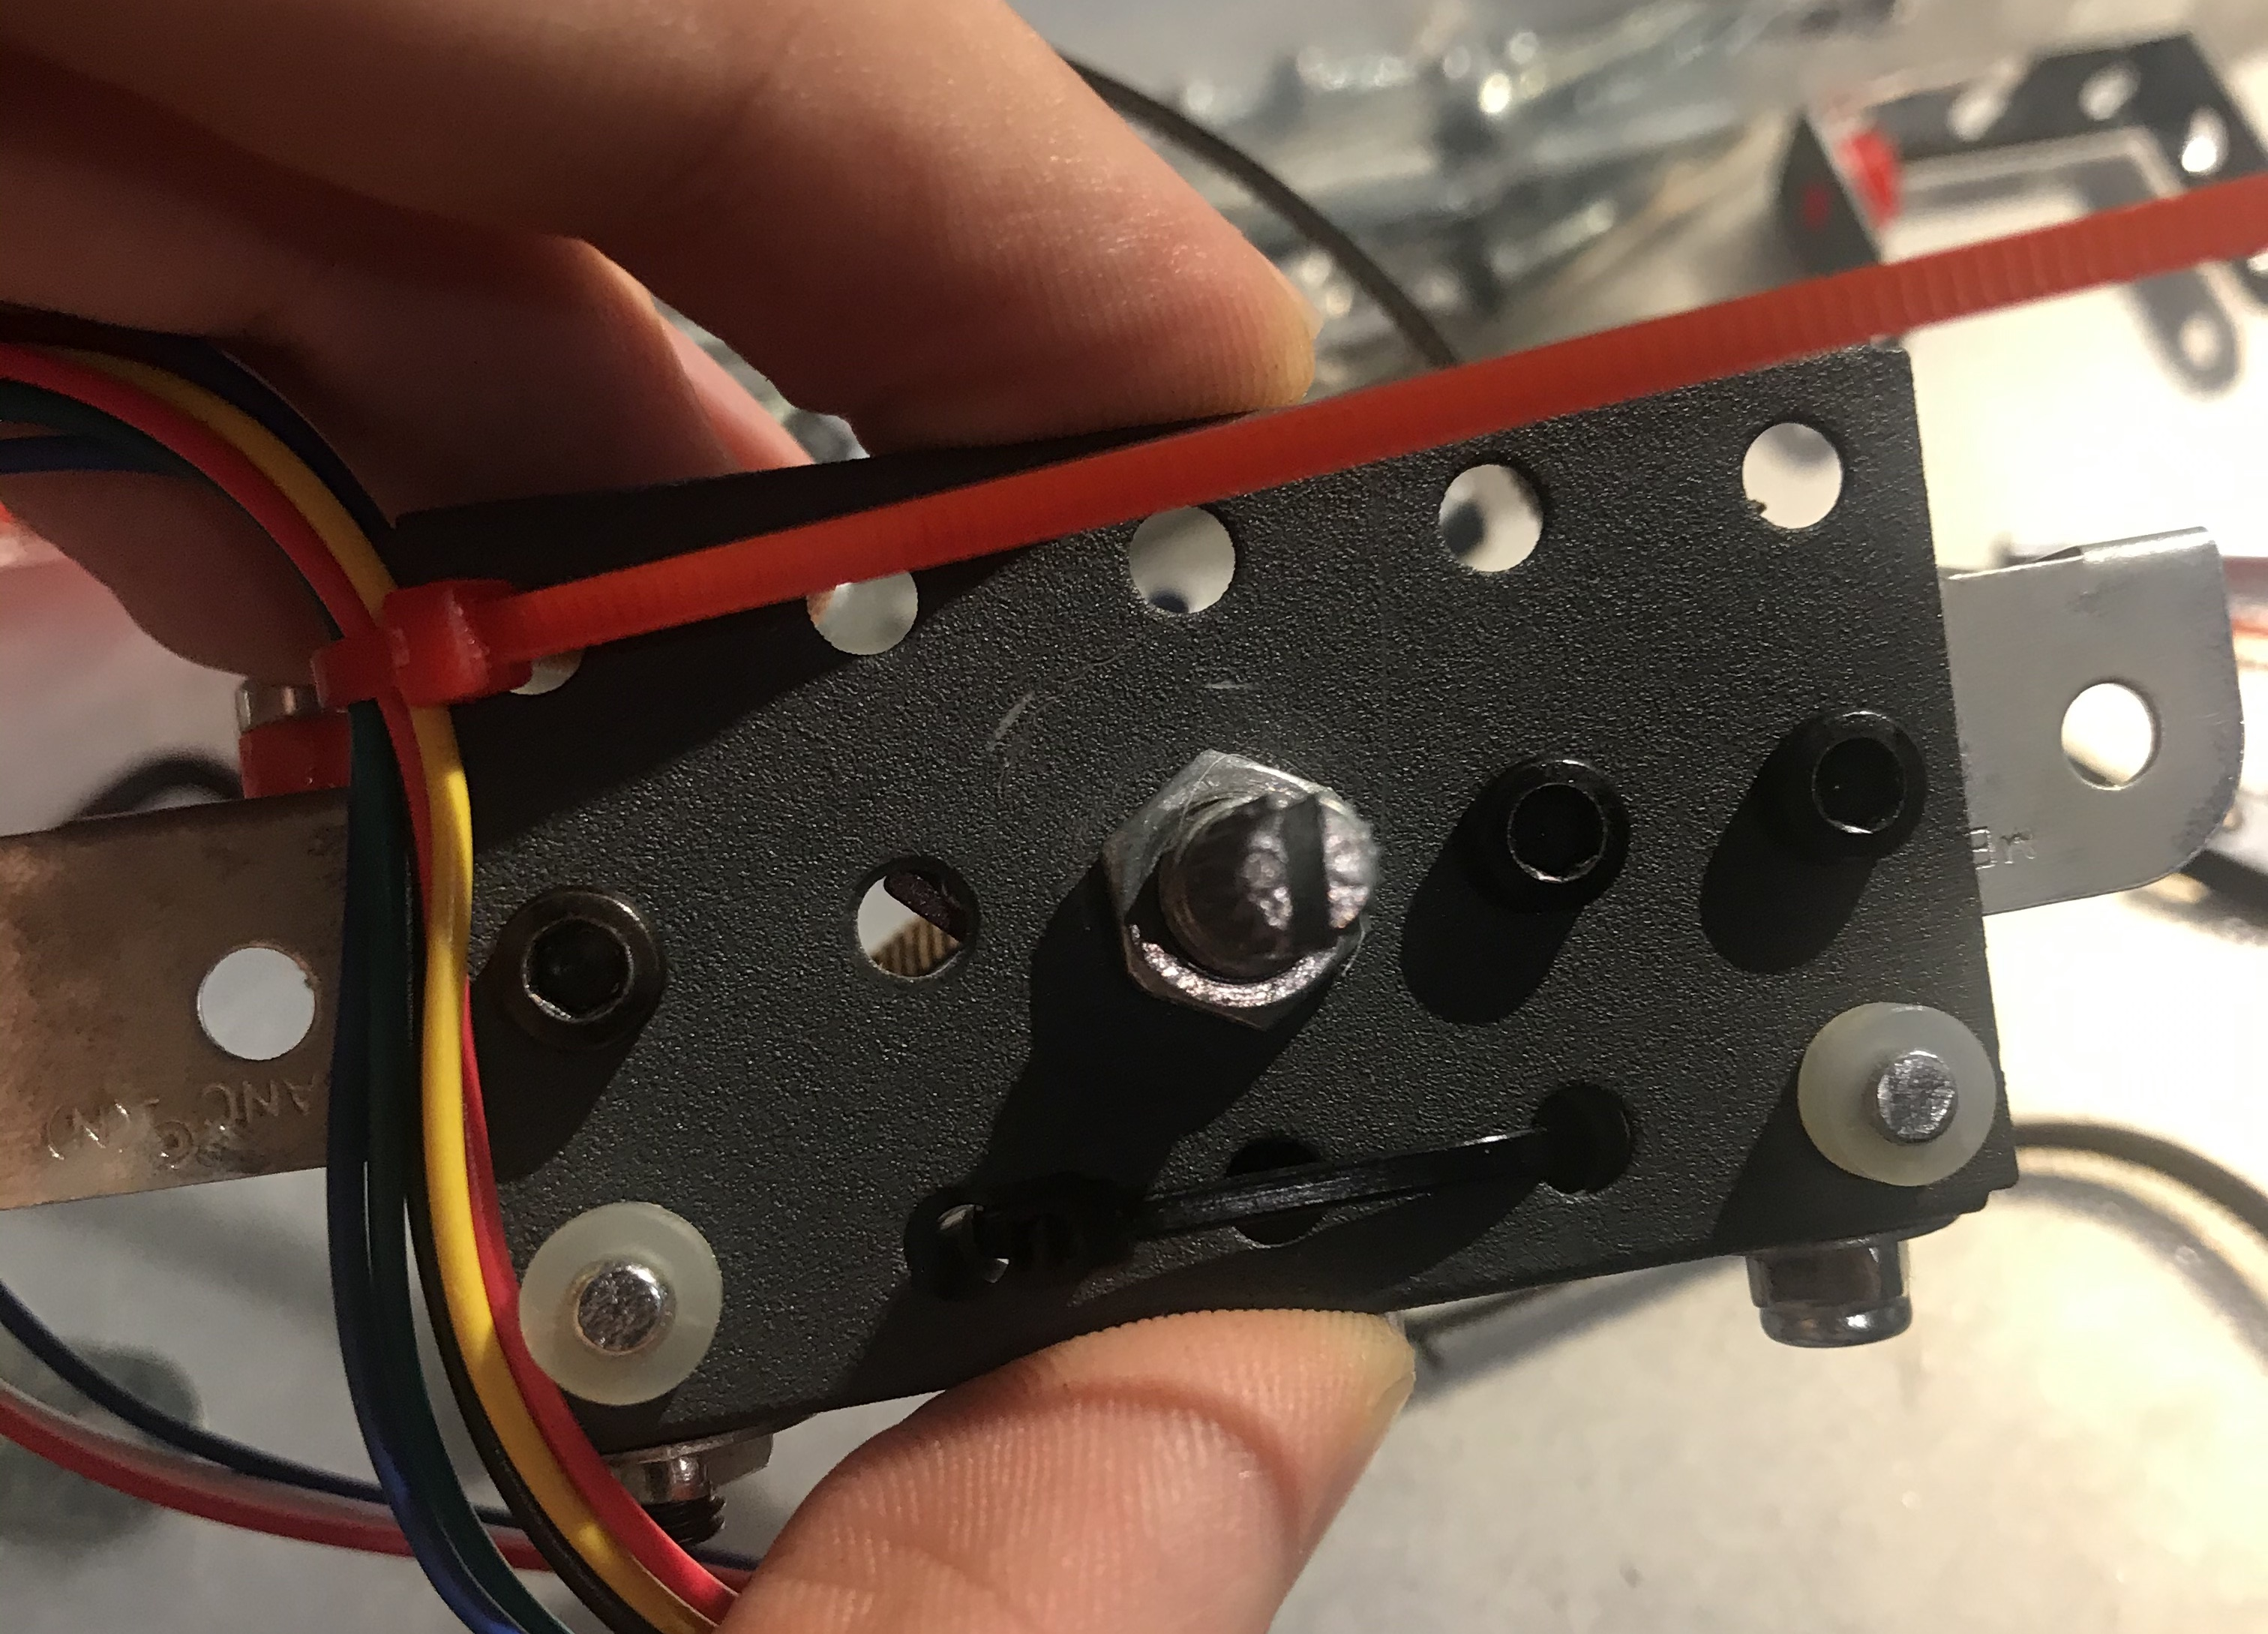
\includegraphics[width=1\linewidth]{figures/IMG_5874.jpg}
  \caption{Potentiometer on Cart}
  \label{fig:cart}
\end{subfigure}%
\begin{subfigure}{.36\textwidth}
  \centering
  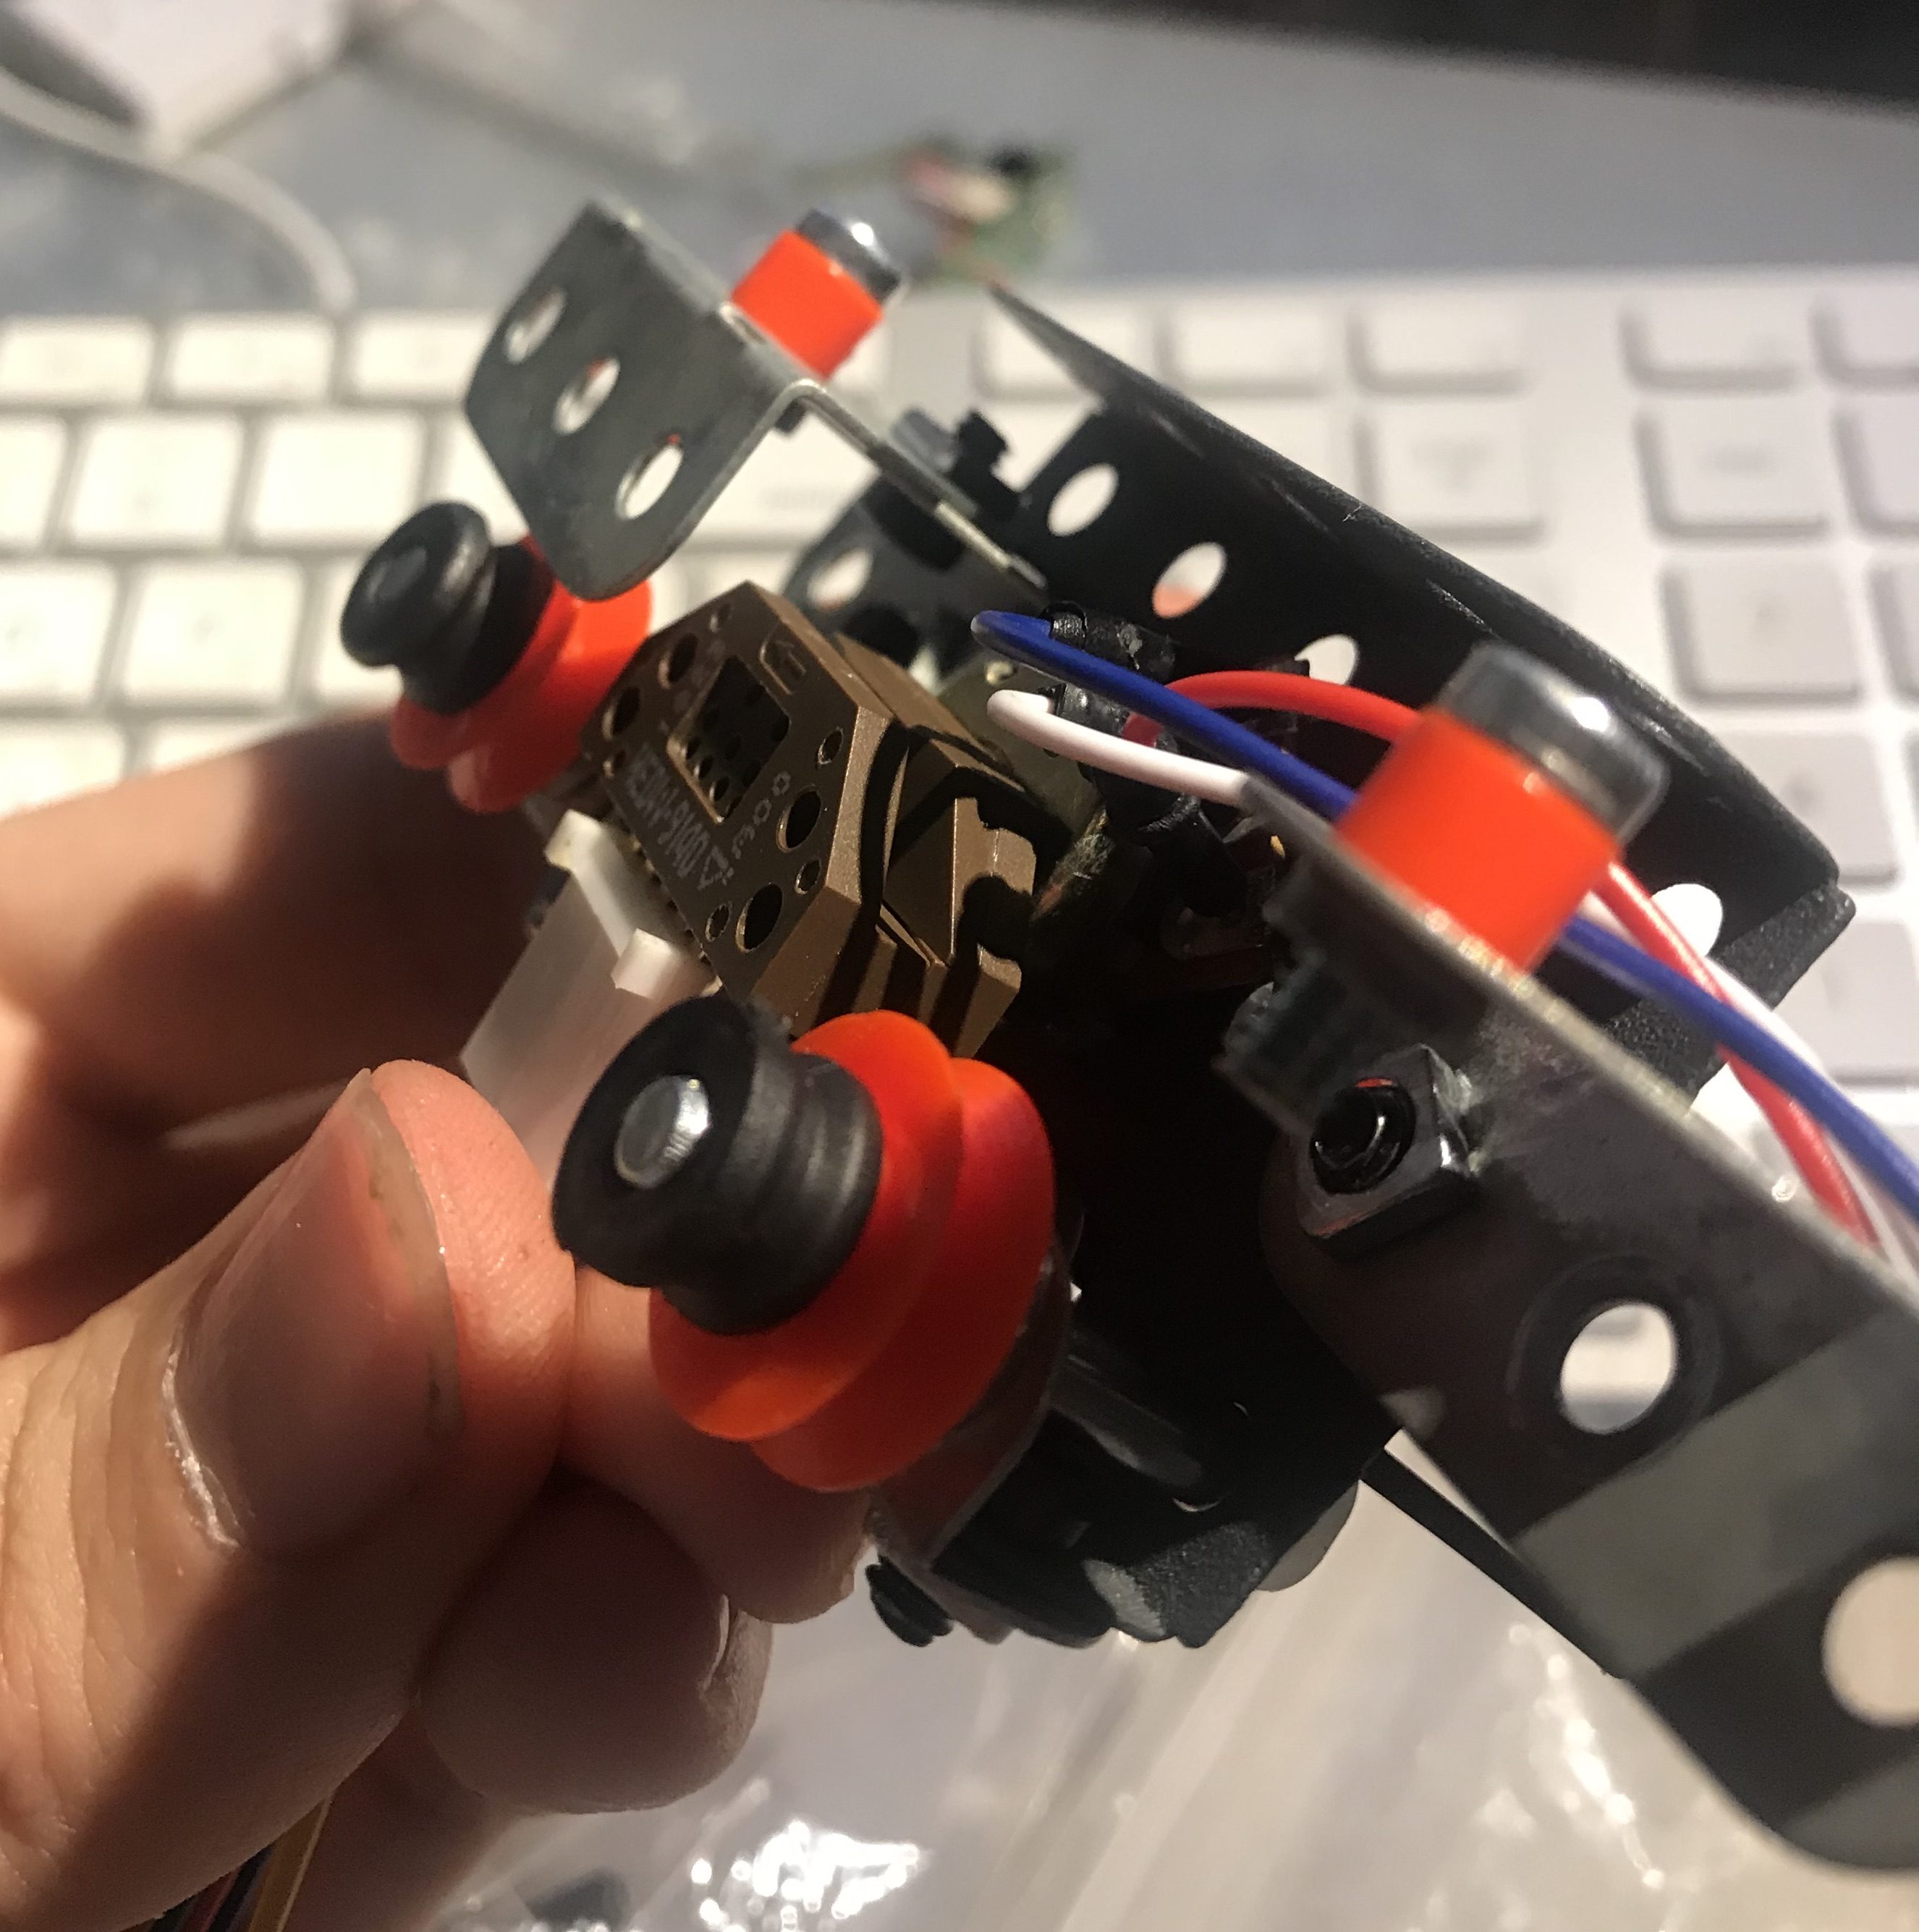
\includegraphics[width=1\linewidth]{figures/IMG_5871.jpg}
  \caption{Optical Encoder on Cart}
  \label{fig:cart2}
\end{subfigure}
\caption{Custom Built Low Friction Linear Guided Cart}
\end{figure}

\subsubsection{Electrical}
The Tiva TM4C123GH6PM microcontroller from Texas Instruments will be used as the real-time embedded controller. Code Composer Studio 9.3.0 for Mac OS X will be used to program and debug the board. A basic breadboard will be used for all wiring connections, and the course H-Bridge motor driver interface board will be used for PWM 12VDC motor control. A circuit drawing can be seen below, where $V_{CC}$ = 3.3V.
\begin{figure}[H]
    \centering
    \begin{tikzpicture}[
                %Global Config
                font=\small
            ]
        %You can create an smart objet like Henry Menke in this post http://www.texample.net/tikz/examples/4-bit-counter/
        % Variables: 1: Position 2: ID.
         \def\TIVA(#1)#2{%
          \begin{scope}[shift={(#1)}]
            \draw[fill=red!10] (-1.5,-2) rectangle (1.5,2); % The body of IC
            \draw[blue] (0,0.6) node [align=center]{TIVA\\TM4C123}; % IC LABEL
            % Draw the pins
            % Some that you have to learn about label nodes, draw lines, and name coordinates in Tikz
            
            
            \draw (0.9,-2) node [above]{GND} -- +(0,-0.5) node [anchor=-45] coordinate (GND); % Pin 1 GND
            %\draw (1.5,0) node [left]{OUT} -- +(0.5,0) node [anchor=-45] coordinate (OUT); % Pin 3 OUT
            \draw (-1.5,1.5) node [right]{PB4} -- +(-0.5,0) node [anchor=-135] coordinate (PB4);
            \draw (-1.5,-0.5) node [right]{PD6} -- +(-0.5,0) node [anchor=-135] coordinate (PD6);
            \draw (-1.5,-1.0) node [right]{PD7} -- +(-0.5,0) node [anchor=-135] coordinate (PD7);
            \draw (1.5,0.0) node [left]{PE4} -- +(0.5,0) node [anchor=-45] coordinate (PE4);
            \draw (1.5,-0.5) node [left]{PE5} -- +(0.5,0) node [anchor=-45] coordinate (PE5);
            
            \draw (0,2) node [below]{$\mathsf{V_{CC}}$} -- +(0,0.5) node [anchor=45] coordinate (VCC2); % Pin 8 VCC
          \end{scope}
        }
        
         \def\HB(#1)#2{%
          \begin{scope}[shift={(#1)}]
            \draw[fill=blue!10] (-1.5,-2) rectangle (1.5,2); % The body of IC
            \draw[blue] (0,0.5) node [align=center]{\large h-Bridge}; % IC LABEL
            % Draw the pins
            % Some that you have to learn about label nodes, draw lines, and name coordinates in Tikz
            
            
            \draw (0.9,-2) node [above]{GND} -- +(0,-0.5) node [anchor=-45] coordinate (GNDHB); % Pin 1 GND
            %\draw (1.5,0) node [left]{OUT} -- +(0.5,0) node [anchor=-45] coordinate (OUT); % Pin 3 OUT
            \draw (-1.5,0.0) node [right]{HB1} -- +(-0.5,0) node [anchor=-135] coordinate (HB1);
            \draw (-1.5,-0.5) node [right]{HB2} -- +(-0.5,0) node [anchor=-135] coordinate (HB2);
            \draw (1.5,0.0) node [left]{M+} -- +(0.5,0) node [anchor=-45] coordinate (M+);
            \draw (1.5,-0.5) node [left]{M-} -- +(0.5,0) node [anchor=-45] coordinate (M-);
            
            \draw (0,2) node [below]{12V} -- +(0,0.5) node [anchor=45] coordinate (12V); % Pin 8 VCC
          \end{scope}
        }
        
        \def\OPT(#1)#2{%
          \begin{scope}[shift={(#1)}]
            \draw[fill=green!10] (-1,-1.5) rectangle (1,1); % The body of IC
            \draw[blue] (-0.5,0.5) node [align=center]{\large Opt.\\Enc.}; % IC LABEL
           
            \draw (1.0,0.0) node [left]{Ch.A} -- +(0.5,0) node [anchor=-45] coordinate (CHA);
            \draw (1.0,-0.5) node [left]{Ch.B} -- +(0.5,0) node [anchor=-45] coordinate (CHB);
            
            \draw (1.0,0.5) node [left]{$\mathsf{V_{CC}}$} -- +(0.5,0) node [anchor=-45] coordinate (VENC);
            \draw (1.0,-1.0) node [left]{GND} -- +(0.5,0) node [anchor=-45] coordinate (GNDENC);
            
          \end{scope}
        }
        
        
        % Start drawing the circuit: Example "Dee-Dah" Siren
        
        % Place the IC's in position
        \TIVA(0,0){1}
        \HB(4,0){1}
        \OPT(-4,-0.5){1}
        %Place polarization nodes:
        \draw (-6,3.5) node[ocirc] (VCC){} node[left]{$\mathsf{V_{CC}}$};
        \draw (-6,-4) node[ocirc] (GND2){} node[left]{GND};
        % Connect U-1
        \draw(VCC) % Start point
            to [short, o-] ++(0.5,0) coordinate (NOD1) % Use auxiliar coordinate (NOD1)
            to [pR, n=POT] (PB4 -| NOD1) % to the point in the intersection between NOD1 and 1 DIS
            to [short] (GND2 -| NOD1)
            to [short] (GND2);
    
        
        %\draw(VCC2) to [short] (VCC);
        \draw(GND) to [short] (GND |- GND2) to [short] (GND2 -| NOD1);
        \draw(GNDHB) to [short] (GNDHB |- GND2)  to [short] (GND |- GND2);
        \draw(GNDENC) to [short] (GNDENC |- GND2);
        \draw[short] (NOD1) -| (VCC2)
        \draw[short] (POT.wiper) -| (PB4)
        \draw(VENC) to [short] (VENC |- VCC);
        \draw[short] (CHA) -| (PD6)
        \draw[short] (CHB) -| (PD7)
        \draw (8,-0.2) node[elmech](motor){M};
        \draw[short] (motor.north) -| (M+)
        \draw[short] (motor.south) -| (M-)
        
        %Place input/output nodes
        % \draw[color=blue,line width=2] (1 TRG) to [short] ++(-0.55,0) node[ocirc] (TRG){} node[below]{Trigger};
        \draw[color=red,line width=2] (12V) to [short] ++(0,0.55) node[ocirc](12V){} node[left]{12V};
    
    \end{tikzpicture}
    

    \caption{Circuit Drawing}
    \label{fig:circ}
\end{figure}



\begin{figure}[H]
    \centering
    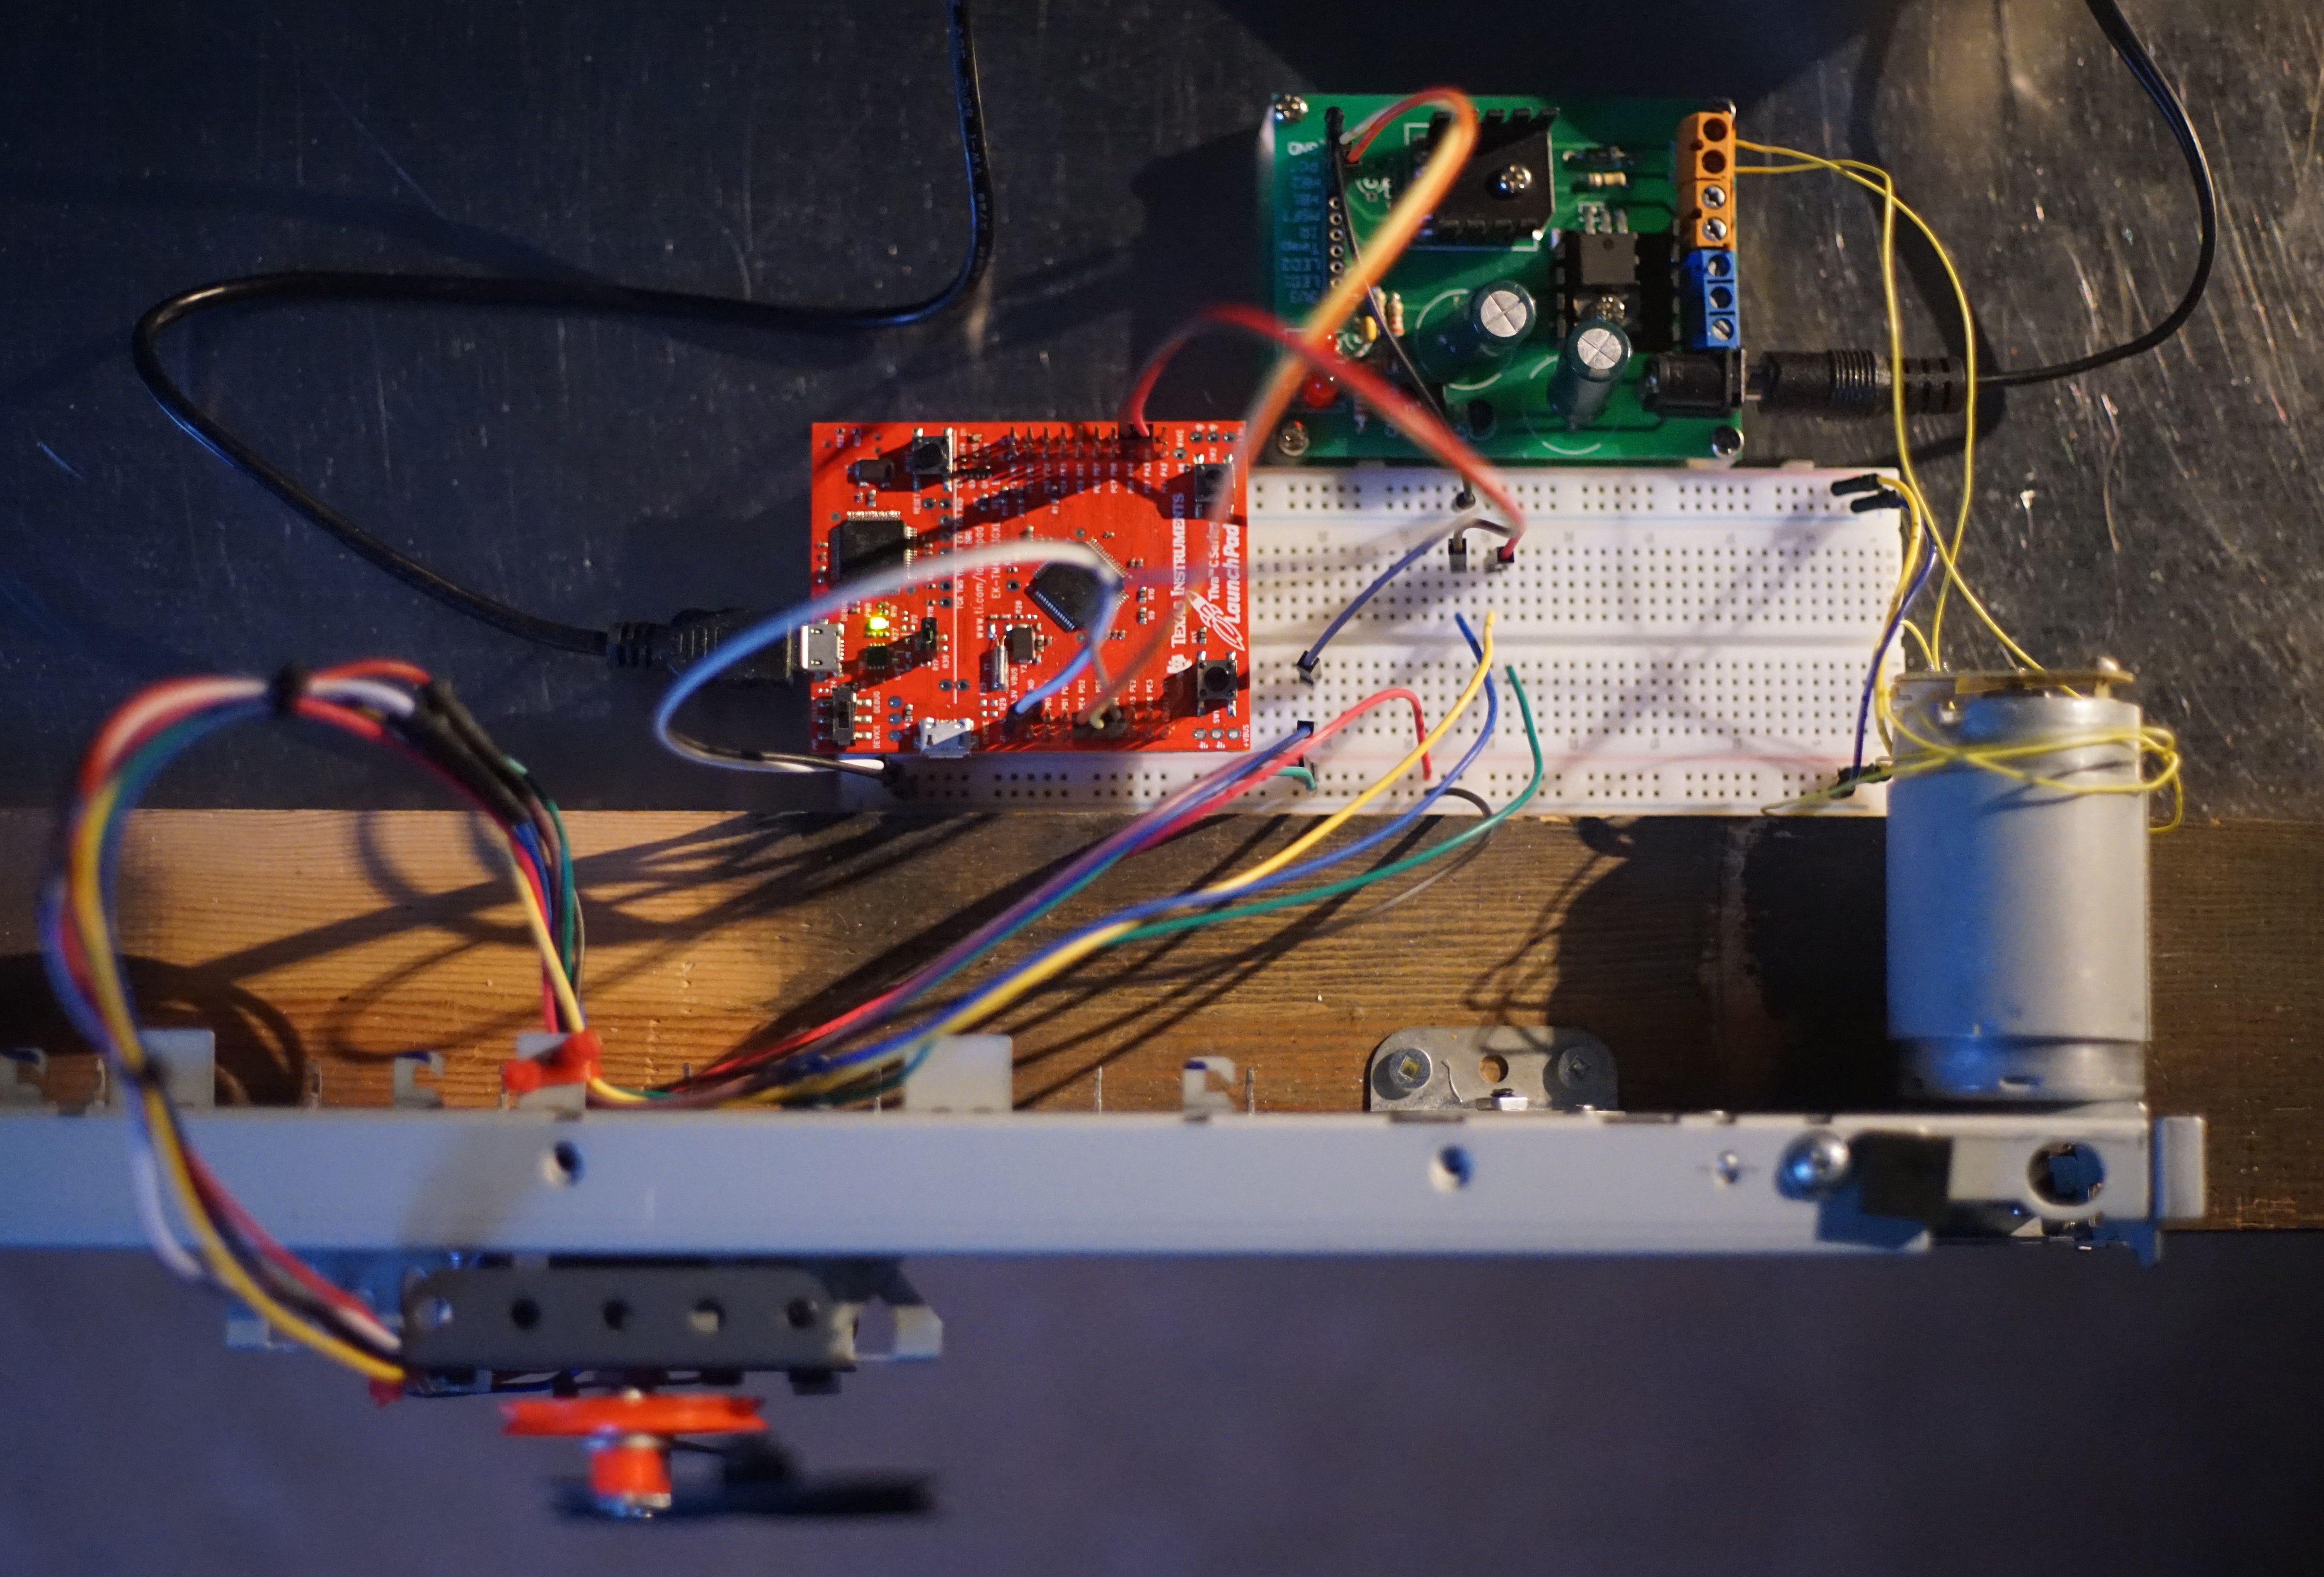
\includegraphics[width=.8\linewidth]{figures/DSC01795.jpg}
    \caption{Completed System Electronics}
    \label{fig:elec}
\end{figure}


\subsubsection{Completed System}
% \begin{figure}
% \centering
% \begin{circuitikz} \draw
% (0,0) to [V, v=$v(t)$, *-*] (0,2) 
%     to [R, l=$R_d$] (2,2)
%     to [L, l=$L_d$] (4,2)
%     to [V, v<=$e(t)$] (4,0) to [generic] (4,2) -- (4,0) -- (0,0);
% \end{circuitikz}
% \end{figure}
% \begin{tikzpicture}
% \ctikzset{tripoles/mos style=arrows}
% \ctikzset{transistors/arrow pos=end}
% \draw(1,-3) to[short] (1,1)
%  (0,-1) to[short] (2,-1)
%  (0,-1.5) to[short] (0,-0.5);
% \draw (0,0) node[npn, ](npn){}; 
% \ctikzset{diodes/scale=0.6}
% \draw (2,-1) to[D, l=$D1$] ++(0,2);
% \draw (0,-2) node[pnp, ](npn){};
% \draw (2,-3) to[D, l=$D2$] ++(0,2);
% \end{tikzpicture}
\begin{figure}[H]
    \centering
    \begin{subfigure}{.49\textwidth}
      \centering
      \includegraphics[width=1\linewidth]{figures/DSC01784.JPG}
      \caption{Complete System}
      \label{fig:comp}
    \end{subfigure}%
    \begin{subfigure}{.49\textwidth}
      \centering
      \includegraphics[width=1\linewidth]{figures/DSC01778.JPG}
      \caption{Linear Cart with Optical Strip}
      \label{fig:compstrip}
    \end{subfigure}
    \caption{Built Inverted Pendulum System}
    \label{fig:invDone}
\end{figure}



\subsection{Software}
To develop the state space model analysis, software tools MATLAB and SIMULINK will be used. MATLAB to develop the system state space model, test and implement state feedback control, and SIMULINK to simulate and observe the system, as well as fine tune the controller gains. Furthermore, the controllability and observability of the system will be assessed in MATLAB.

\subsubsection{Control System Flowchart}

% Define block styles
\tikzstyle{decision} = [diamond, draw, fill=green!20, 
    text width=4.5em, text badly centered, node distance=3cm, inner sep=0pt]
\tikzstyle{block} = [rectangle, draw, fill=blue!20, 
    text width=5em, text centered, rounded corners, minimum height=4em]
\tikzstyle{line} = [draw, -latex']
\tikzstyle{cloud} = [draw, ellipse,fill=red!20, node distance=3cm,
    minimum height=2em]

\begin{figure}[H]
    \centering
    \footnotesize
    \begin{tikzpicture}[node distance = 2cm, auto]
    
        % Place nodes
        \node [block] (init) {initialize system};
        \node [cloud, left of=init] (obsvh) {obsv.h};
        \node [cloud, right of=init, node distance=6cm] (hand) {peripherals, ISRs};
        \node [block, below of=init] (eval) {evaluate inputs};
        \node [decision, below of=eval] (decide) {conditions met and timer interrupt?};
        \node [block, below of=decide, node distance=3cm] (eval2) {evaluate inputs};
        \node [block, left of=eval2, node distance=3cm] (dc0) {set 0\% duty cycle};  
        \node [block, below of=dc0, node distance=2cm] (loop2) {loop};  
        \node [block, below of=eval2, node distance=2cm] (obsv) {run observer};
        \node [block, below of=obsv, node distance=2cm] (dc) {LQR $\implies$ duty cycle};
        \node [block, below of=dc, node distance=2cm] (loop) {loop};
        \node [block, below of=hand, node distance=2cm] (pf) {port f handler};
        \node [block, below of=pf, node distance=2cm] (uart) {UART handler};
        \node [block, below of=uart, node distance=2cm] (qei) {QEI};
        \node [block, below of=qei, node distance=2cm] (adc) {ADC};
        \node [block, below of=adc, node distance=2cm] (timer) {timer handler};
        
        % Draw edges
        \path [line] (init) -- (eval);
        \path [line] (eval) -- (decide);
        \path [line] (decide) -- node {yes}(eval2);
        \path [line] (eval2) -- (obsv);
        \path [line] (obsv) -- (dc);
        \path [line] (dc) -- (loop);
        \path [line] (dc0) -- (loop2);
        \path [line] (loop.east) -- ++(1.5,0) -- ++(0,1.5) -- ++(0,7.5) -- (decide.east);
        \path [line] (loop2.west) --  ++(-1.5,0) -- ++(0,2) -- ++(0,6) -- (eval.west);
        \path [line] (decide) -| node [near start] {no} (dc0);
        \path [line,dashed] (obsvh) -- (init);
        \path [line,dashed] (init) -- (hand);
        \path [line,dashed] (hand.east) |- (pf.east);
        \path [line,dashed] (hand.east) |- (uart.east);
        \path [line,dashed] (hand.east) |- (qei.east);
        \path [line,dashed] (hand.east) |- (adc.east);
        \path [line,dashed] (hand.east) |- (timer.east);
        %\path [line,dashed] (obsvh) |- (eval);
        
    \end{tikzpicture}

    \caption{Controller Flowchart}
    \label{fig:flow}
\end{figure}

\subsubsection{LQR Control Implementation}
In order to effectively run the full state feedback controller, calculation of \textit{u} must be done at a specified frequency, rather than at the variable CPU crystal frequency of 80MHz, which is far too fast. The algorithm can be seen below, with exponential filters applied to smooth the noisy data and derivatives.\\
\footnotesize
\begin{algorithm}[H]
    \SetAlgoLined
    \SetKwInOut{Input}{Input}
    \SetKwInOut{Output}{Output}
    \Input{Measured states, $x$}
    \Output{Estimated states, $\hat{x}$}
    Calculates $\dot{x}$ and $\dot{\theta}$ based off measurements of $x,\theta$ and exponential smoothing\\
    rPosDot = 0.05\\
    rThetaDot = 0.02\\
    rTheta = 0.15\\
    \bigskip
    $\hat{x}.X = (x - x_{ref})scale_x$\\
    $\hat{x}.Y = (1-rPosDot)\dot{x}_{k-1} + rPosDot(\hat{x}.X - x_{k-1})/dt$\\
    $\hat{x}.Z = (1-rTheta)\theta_{k-1} + rTheta(\theta_{max}-readADC() - \theta_{ref})scale_\theta$\\
    $\hat{x}.W = (1-rThetaDot)\dot{\theta}_{k-1} + rThetaDot(\hat{x}.Z - \theta_{k-1})/dt$\\
    $x_{k-1} = \hat{x}.X$\\
    $\dot{x_{k-1}} = \hat{x}.Y$\\
    $\theta_{k-1} = \hat{x}.Z$\\
    $\dot{\theta_{k-1}} = \hat{x}.W$\\
    
    \caption{Full State Calculation Algorithm}
\end{algorithm}
\normalsize
This algorithm implementation in C can be seen in appendix \ref{lqrctrl}. Following this calculation, the duty cycle of the motor is set via this equation.
\begin{equation}
    u = -Kx \implies dc = -\alpha_{dc} K \hat{x}
\end{equation}
Where $\alpha_{dc}$ is a tuned constant that scales the input \textit{u} to the required duty cycle levels, which range from -50000 to 50000.
\subsubsection{Luenberger Observer Implementation}
To elaborate on our control model approach shown in figure \ref{fig:fc}, the following algorithm will be implemented in C to estimate the immeasurable states, $\dot{x}, \dot{\theta}$, the velocity of the cart and the rotational velocity of the pendulum.\\

\footnotesize
\begin{algorithm}[H]
    \SetAlgoLined
    \SetKwInOut{Input}{Input}
    \SetKwInOut{Output}{Output}
    \Input{Measured states, $x$}
    \Output{Estimated states, $\hat{x}$}
    Update observer state estimator global variables $\dot{x},\dot{\theta}$\\
    Based off measurements of $x,\theta$\\
    \bigskip
    $dt = 1/CtrlFreq$\\
    $y = Cx$\\
    \While{\|e\| \geq \tau}{
        $\hat{y} = C\hat{x}$\\
        $e = y - \hat{y}$\\
        $\dot{\hat{x}} = (A-BK)\hat{x} + Le$\\
        $\hat{x_{n}} = \hat{x} + \dot{\hat{x}}dt$\\
        $\hat{x} = \hat{x_{n}}$\\
        }
    \caption{Luenberger Observer Algorithm}
\end{algorithm}
\normalsize
This algorithm implementation in C can be seen in appendix \ref{obsverver}.

\section{Results}
\subsection{MATLAB Simulation Results}
After completing the state model for the linearized system, the model was then implemented and simulated in MATLAB. This allows for software-in-the-loop testing of the system, without the concerns of breaking hardware, sensor noise, non-linearities and more. However, this can pose as a risk as the system simulation accuracy cannot be exact, due to said non-linearities that only exist in a physical system, such as friction, motor back EMF, and more. 
\subsubsection{Impulse Responses}
An example plot of the system's impulse response can be seen below. This plot was output upon every tune of the gain matrix \textit{K} to ensure stable disturbance rejection.
\begin{figure}[H]
    \centering
    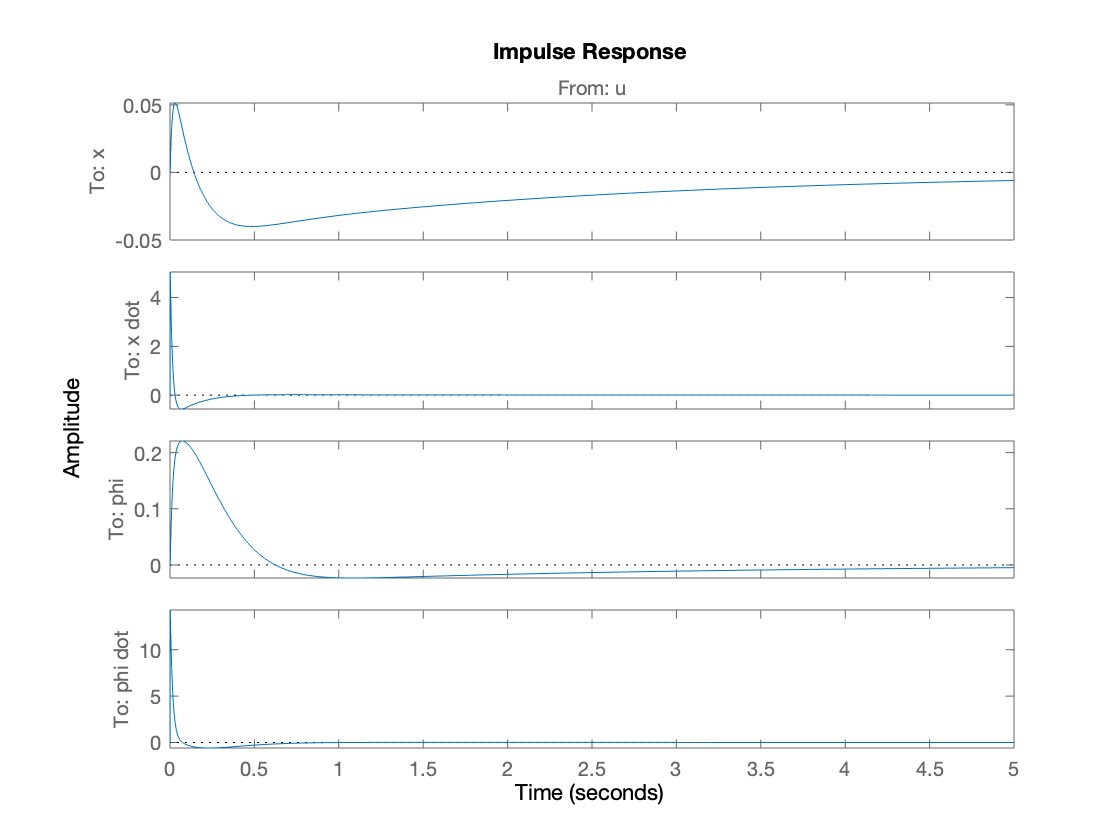
\includegraphics[width=0.7\linewidth]{figures/impulse.png}
    \caption{State Feedback System Impulse Response in MATLAB}
    \label{fig:imp}
\end{figure}

\subsubsection{Step Response}
Figure \ref{fig:sim} shows an example of the simulated discrete time system response for a cart position step input of \textit{20cm}.
\begin{figure}[H]
    \centering
    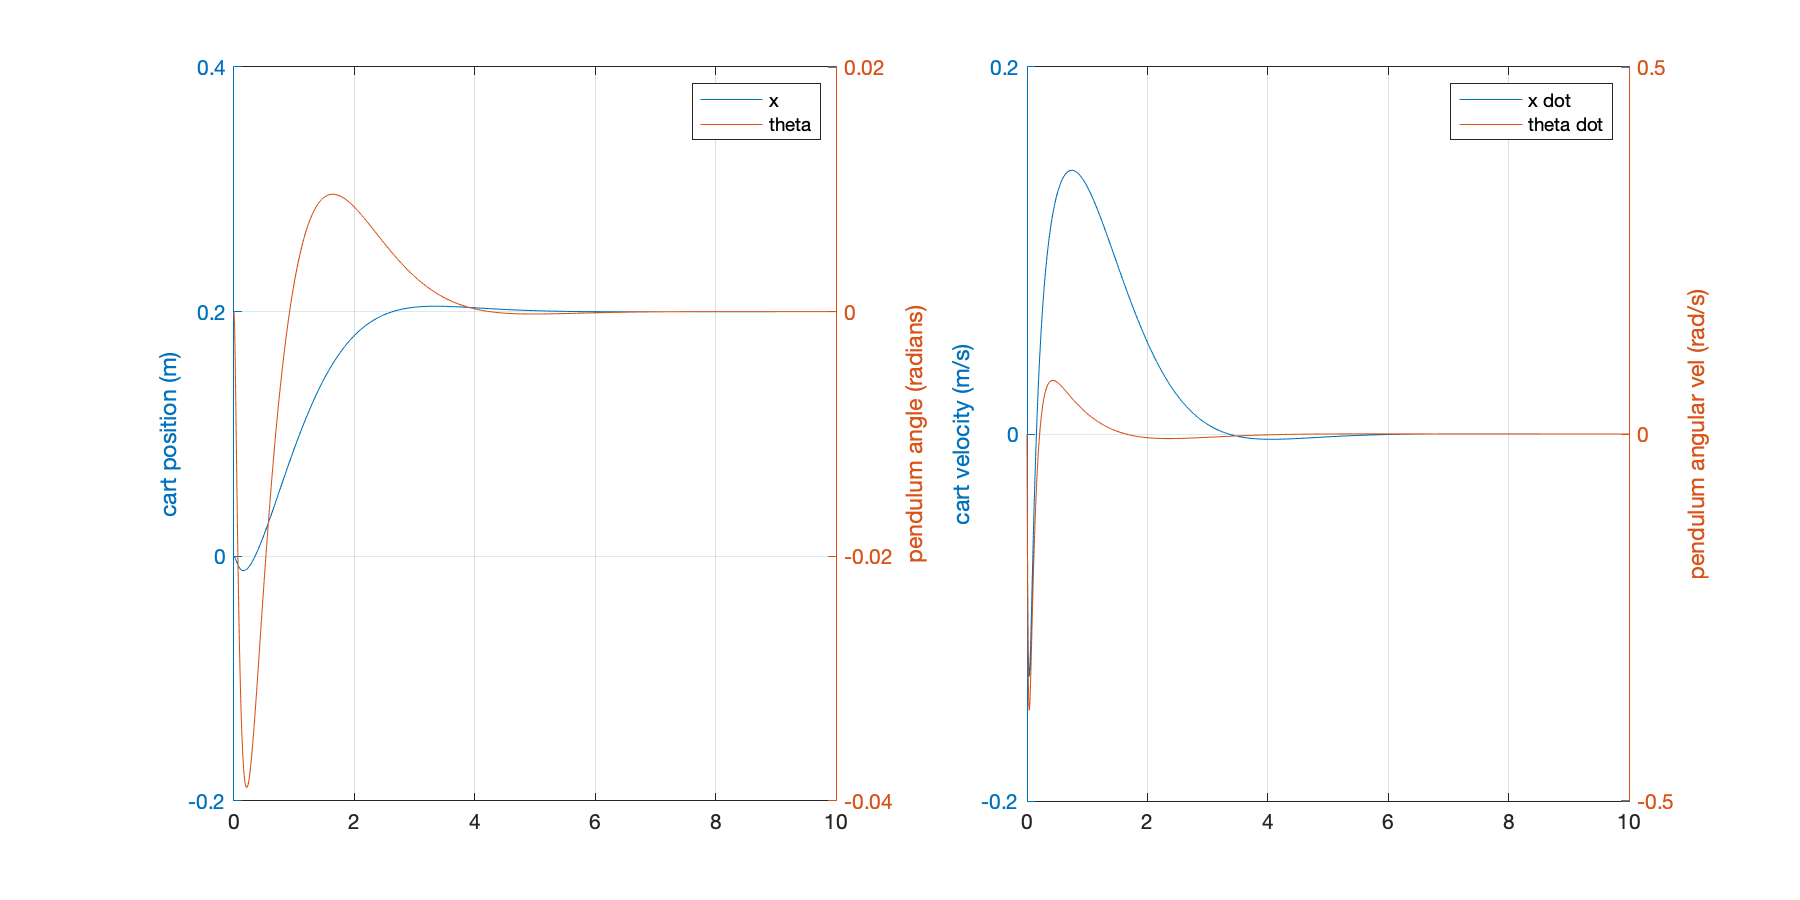
\includegraphics[width=1\linewidth]{figures/models.png}
    \caption{Observer Based State Feedback System Step Response in MATLAB}
    \label{fig:sim}
\end{figure}
\subsection{SIMULINK Models}
SIMULINK was also used to build simulation models, in addition to MATLAB's functions. This was to ensure feasible testing of tuning prior to implementation on the physical system.
\subsubsection{Full State Feedback}
\begin{figure}[H]
    \centering
    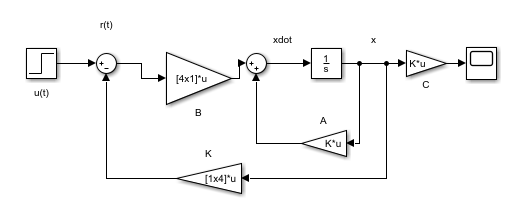
\includegraphics[width=0.7\linewidth]{figures/Feedback.PNG}
    \caption{SIMULINK State Feedback Controller Model}
    \label{fig:sim}
\end{figure}
\subsubsection{Observer Based}
\begin{figure}[H]
    \centering
    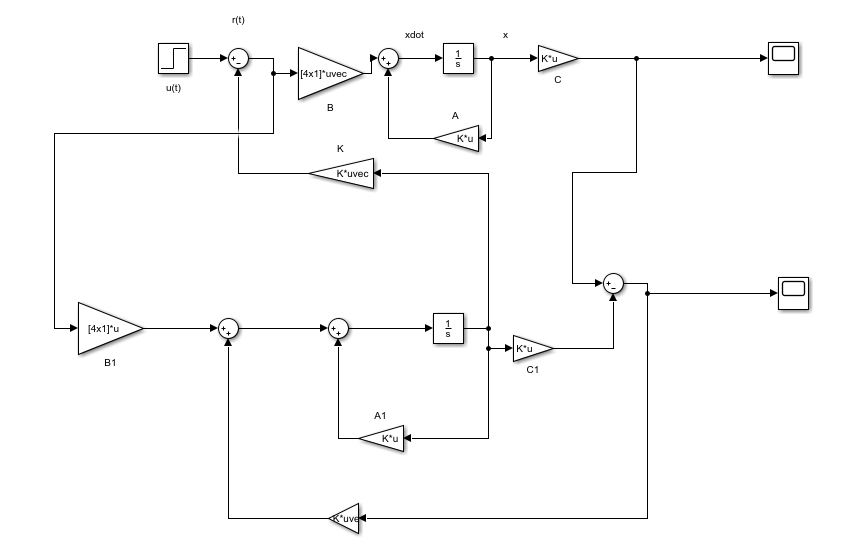
\includegraphics[width=0.9\linewidth]{figures/obs.PNG}
    \caption{SIMULINK Observer Based State Feedback Controller Model}
    \label{fig:sim}
\end{figure}
\subsection{Experimental Results}
Overall, the physical system is very controllable. Adequate sensors and a powerful motor enable the robust, real time embedded control of the inverted pendulum system. However, there are limitations to tuning the physical system based off a state space model of the system whose variables, though measured, may not account for all the non-linearities that exist in a practical, physical control system. Nonetheless, the following sections discuss the overall system tuning results. Responses have been plotted in MATLAB through serial UART communication with the tiva microcontroller for a more in depth analysis.

\subsubsection{Gain Tuning Process}
Once the system was completely setup and tested with PID control, development and testing of the observer had to be streamlined. Rather than tuning in MATLAB, copying and pasting system matrices, a function was developed in MATLAB to export the \textit{obsv.h} file, containing said constants. This file can be seen in appendix \ref{obsvh}.

\begin{figure}[H]
    \centering
    \footnotesize
    \begin{tikzpicture}[node distance = 2cm, auto]
    
        % Place nodes
        \node [block] (model) {initialize model};
        \node [cloud, above of=model, node distance=2.5cm] (system) {system model};
        \node [block, right of=model, node distance=2.5cm] (tune) {tune \textit{K, L} in matlab};
        \node [block, right of=tune, node distance=2.5cm] (export) {export model (\textit{obsv.h})};
        \node [block, right of=export, node distance=2.5cm] (test) {test tiva system};
        \node [decision, right of=test] (tuned) {tuned, stable system?};
        \node [cloud, right of=tuned] (done) {done};
        
        % Draw edges
        \path [line] (system) -- (model);
        \path [line] (model) -- (tune);
        \path [line] (tune) -- (export);
        \path [line] (export) -- (test);
        \path [line] (test) -- (tuned);
        \path [line] (tuned) -- node {yes}(done);
        \path [line] (tuned.south) -| node {no}(model.south);
    \end{tikzpicture}

    \caption{Tuning Process Flowchart}
    \label{fig:tune}
\end{figure}

\subsubsection{Basic P Controller - PID Control}
To observe functioning and successful system integration, a basic P controller was first implemented. Figure \ref{fig:step} displays the measured states $x, \theta$, of the system through UART communication with MATLAB as the pendulum responds to minor impulses. Let it be noted that a second impulse returned the cart to the reference positon, $x=0cm$.
\begin{figure}[H]
    \centering
    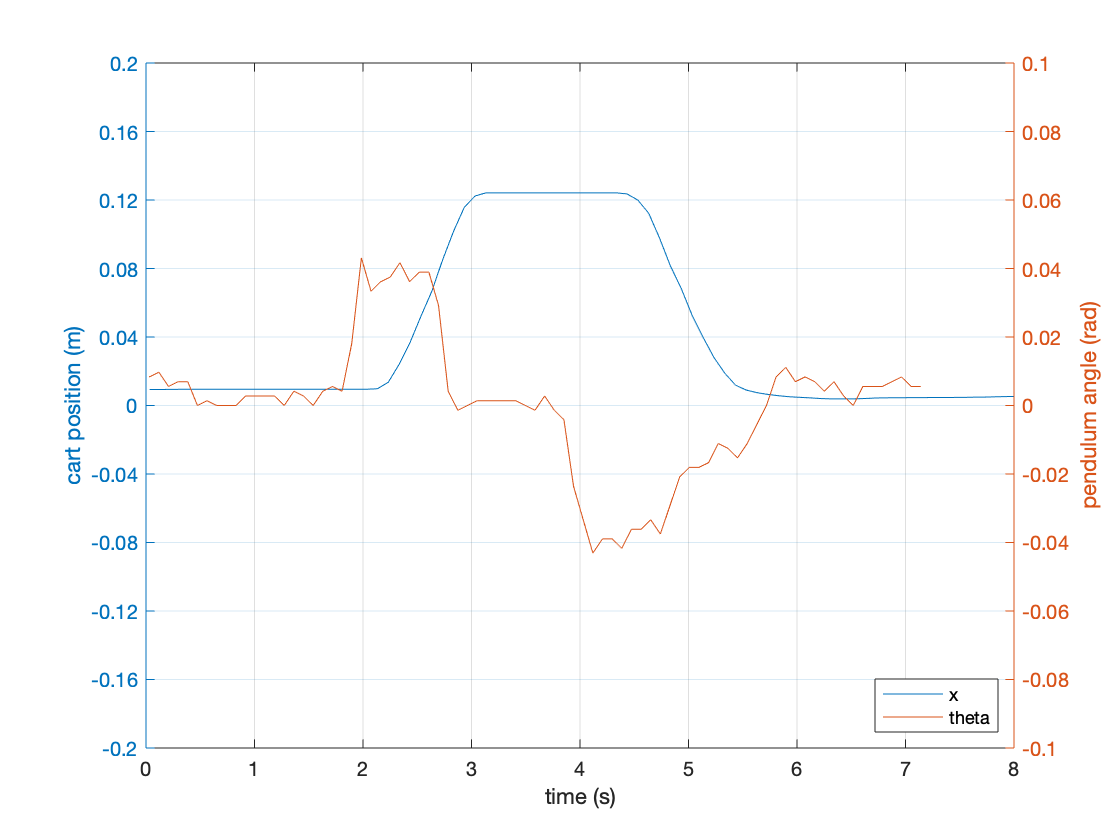
\includegraphics[width=.7\linewidth]{figures/nice.png}
    \caption{Physical System Response}
    \label{fig:step}
\end{figure}
It can be seen above that as the pendulum angle moves further from 0, the cart's position is adjusted by the motor in order to ensure the pendulum remains stable. At most, the pendulum angle moves 0.08 radians, approximately 4.58$^o$, which satisfies the controller requirements. Moreover, a settling time of $\leq$ 4 seconds is clear, however there exists steady state error with respect to the cart's position. After a quick analysis of controllability of an inverted pendulum using PID control, it can be seen that there will always exist steady state error for the cart position \cite{pidBad}, which will also be very unstable, hence the demand for a state feedback type controller.
\\\\
After the manual tuning method was implemented, the system ended up with a relatively satisfactory proportional gain for a P controller. As the gain for P ($K_P$) increases, the most observable effects are the decrease in rise time, increase in overshoot, decrease in steady state error, and a degrade in the stability of the system with an overall small change in settling time. After the manual manipulation of $K_P$, the settled upon gain after a few attempts was a value of $800$.  
\subsubsection{LQR Full State Feedback Control}
After initial implementation of a state feedback controller, tuned via LQR methods in MATLAB, it was found that the pendulum was quite stable, however the cart would easily oscillate about it's set point (reference) upon any disturbances, even just sensor noise would cause it to oscillate. Figure \ref{fig:osc} displays the cart's position in red, upon a minor disturbance to the pendulum.
\begin{figure}[H]
    \centering
    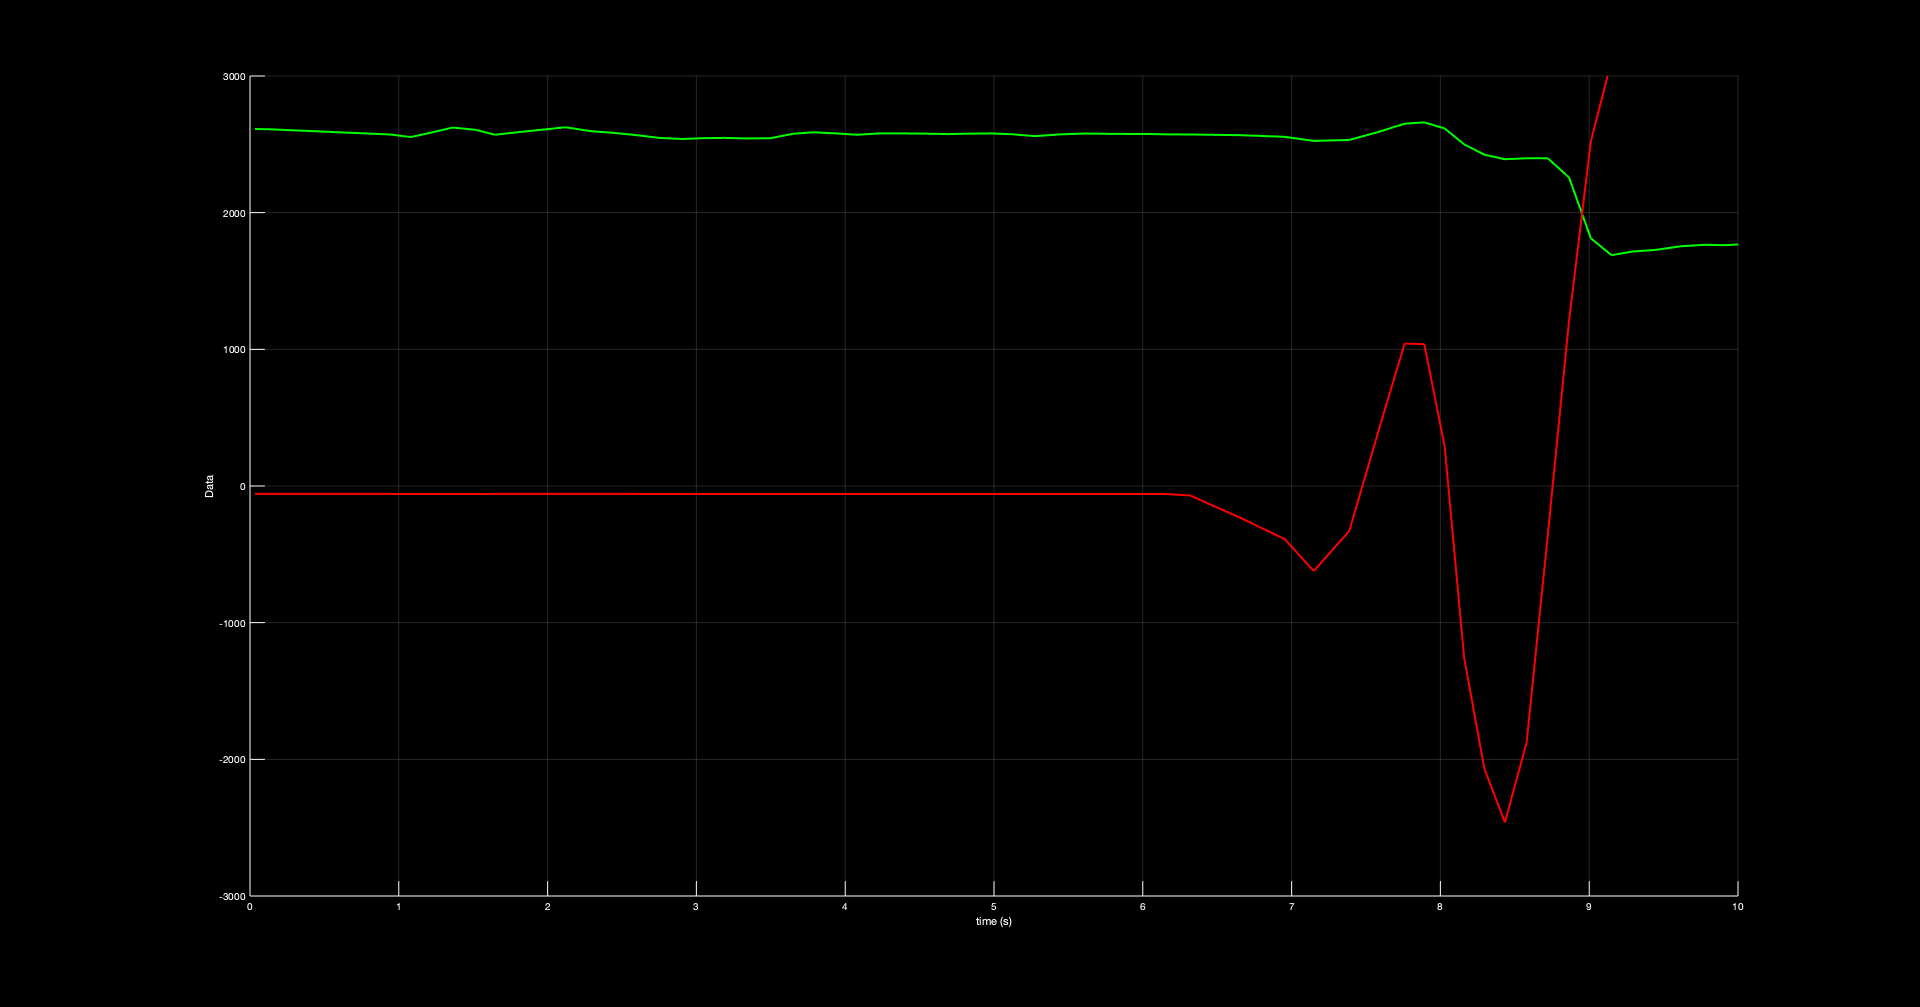
\includegraphics[width=.6\linewidth]{figures/posOsc2withDotStates.png}
    \caption{Cart Oscillation}
    \label{fig:osc}
\end{figure}
While tuning the system in MATLAB using the \textbf{lqr} function, it was found that the system tuning for a continuous time system, while in reality our physical system is implemented on a microprocessor, hence it is a discrete time system. Thus, use of the \textbf{dlqr} command on the state model improved placement of the closed loop poles to within the unit circle or the s-plane.
\begin{figure}[H]
    \centering
    \begin{subfigure}{.49\textwidth}
      \centering
      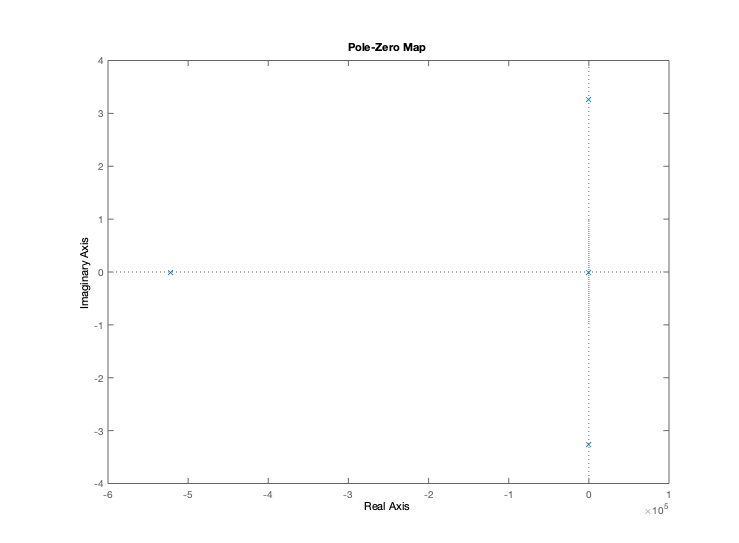
\includegraphics[width=1\linewidth]{figures/pzBigLQR.png}
      \caption{Pole Placement with \textbf{lqr}}
    \end{subfigure}
    \begin{subfigure}{.49\textwidth}
      \centering
      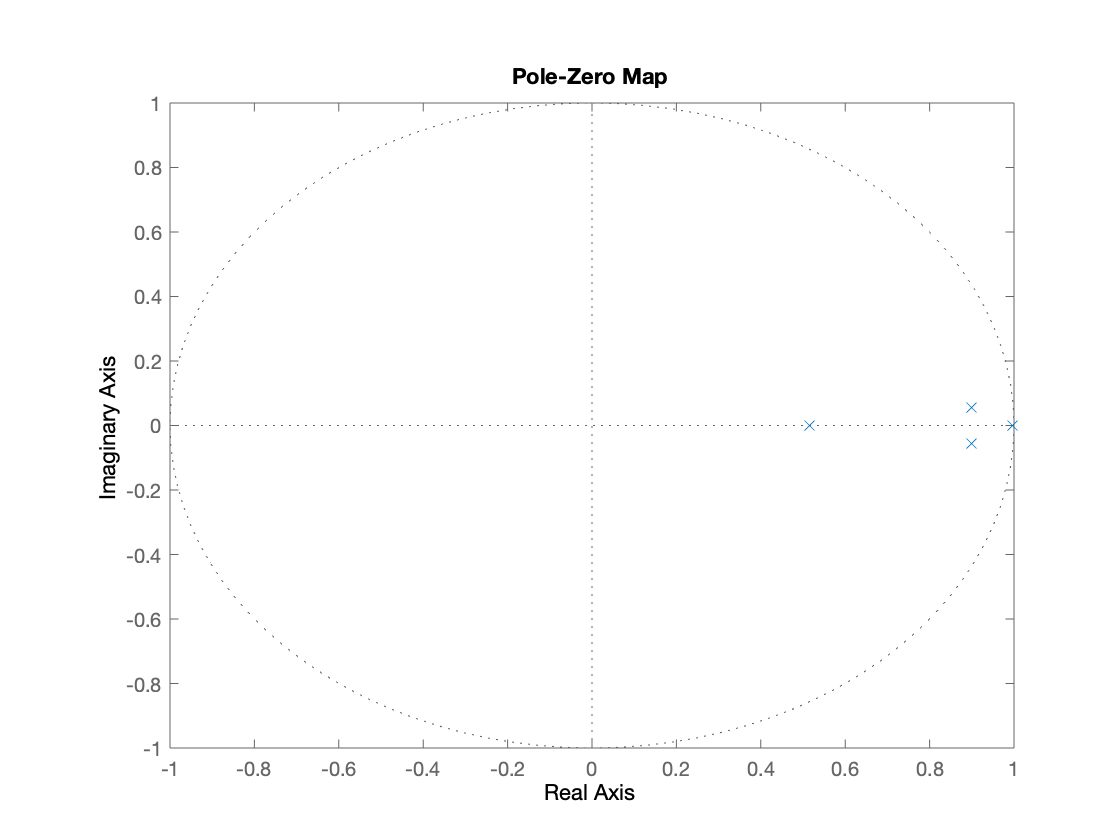
\includegraphics[width=1\linewidth]{figures/dlqrPoles.png}
      \caption{Pole Placement with \textbf{dlqr}}
    \end{subfigure}
    \caption{MATLAB Pole Placement via LQR}
    \label{fig:lqrPoles}
\end{figure}
As seen in figure \ref{fig:lqrPoles}, the continuous time system on the left has an incredibly aggressive pole below $-5x10^5$, whereas the digital tuning has practical poles. Physically, this resulted in a much more stable system. Minor impulses to the cart did not have as great of an effect as before. This is because pole placement theory is different for continuous and discrete time cases, as shown in the figure below.
\begin{figure}[H]
    \centering
    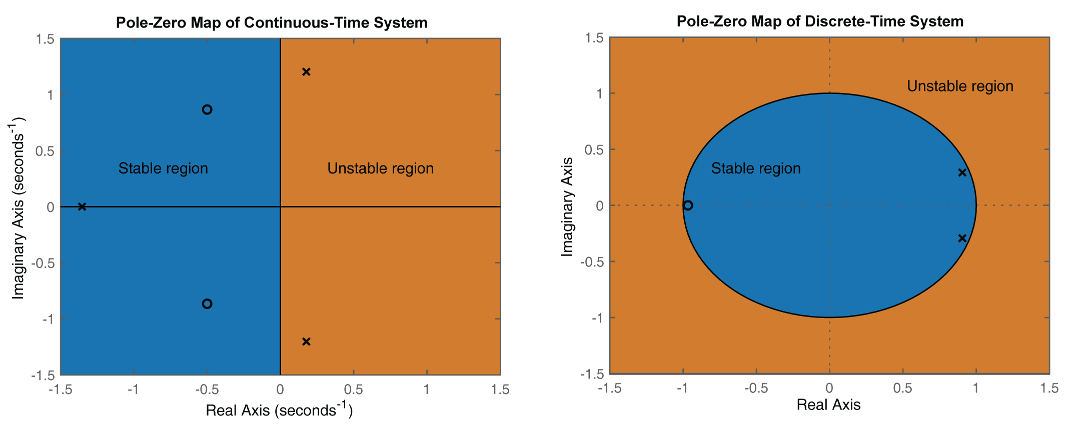
\includegraphics[width=.8\linewidth]{figures/dtpoles.png}
    \caption{Continuous vs Discrete Time Pole Placement \cite{pz}}
    \label{fig:pz}
\end{figure}
Testing with MATLAB functions \textbf{place} and \textbf{acker} proved to result in incredibly large values of \textit{K}, that also placed far too much control effort on the cart position \textit{x}, hence these commands could not be used. After some testing with the \textbf{dlqr} function, the following optimal values were obtained for \textit{K}.
\begin{equation}
    Q =
    \begin{bmatrix}
    1000 & 0 & 0 & 0\\
    0 & 0 & 0 & 0\\
    0 & 0 & 5000 & 0\\
    0 & 0 & 0 & 0
    \end{bmatrix},
    R = 1 \implies K = [-27.7730,-9.4171,66.4014,5.0086]
\end{equation}
However, these values for K are still not completely optimal, but are a great base for \textit{K}. Even still, the cart seems to oscillate about it's reference point, while keeping the pendulum inverted, similar to that of figure \ref{fig:osc}. After some manual tuning of K, the following values optimized the performance of the system.
\begin{equation}
    K = [-25.0,-20.0,40.0,5.0]
\end{equation}
\begin{figure}[H]
    \centering
    \begin{subfigure}{.49\textwidth}
      \centering
      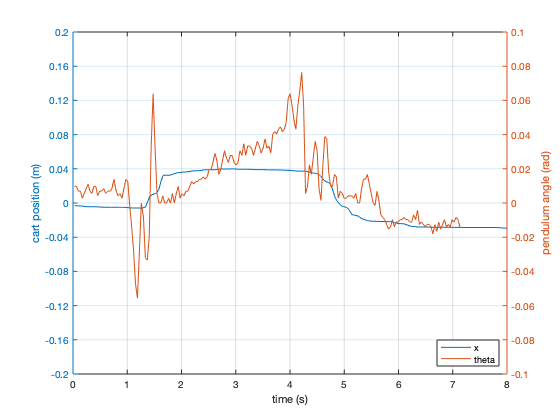
\includegraphics[width=1\linewidth]{figures/decent.png}
      \caption{Decent Tune}
    \end{subfigure}
    \begin{subfigure}{.49\textwidth}
      \centering
      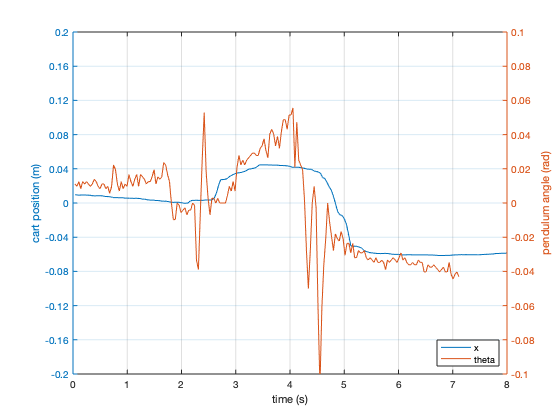
\includegraphics[width=1\linewidth]{figures/best.png}
      \caption{Better Tune}
      \label{fig:best}
    \end{subfigure}
    \caption{Final System Response to Disturbance Rejection}
    \label{fig:finals}
\end{figure}
However, there is still too much oscillation of the cart. This is due to the gain $k_2$, which amplifies the cart velocity, $\dot{x}$, hence it was turned down just enough. The response can be seen above in figure \ref{fig:best}.
\begin{equation}
    K = [-25.0,-18.0,40.0,5.0]
\end{equation}
Clearly, the cart did not finish at it's reference position of $x=0cm$, instead it shot past by $6cm$. Steady state error can be eliminated by adding a pre-compensator, an integrator, or a Luenberger observer, which is discussed in the following section.
\subsubsection{Observer Based State Feedback Control}
Unfortunately due to project time constraints, the observer was never properly implemented. After hours of testing, gains could not be tuned to drive $e \implies 0$. Thus, the system was very unstable. Tuning was done in MATLAB, with placement of observer poles ~5 times faster than the system closed loop poles. All implementation is present, however a proper \textit{L} must be found to achieve a functioning observer. 

\subsection{Additional System Enhancements}
This section outlines the modifications that were made to the system to solve problems that were discovered throughout the development of the project.

\subsubsection{Potentiometer Short Circuiting}
After tireless troubleshooting it was found that there was a faulty connection in the wiring for the potentiometer. The following figures display the noise induced by this error, and it's effect on the system performance. It can be seen that the cart was incredibly 'jumpy' prior to the re-wiring of the sensor.
\begin{figure}[H]
    \centering
    \begin{subfigure}{.49\textwidth}
      \centering
      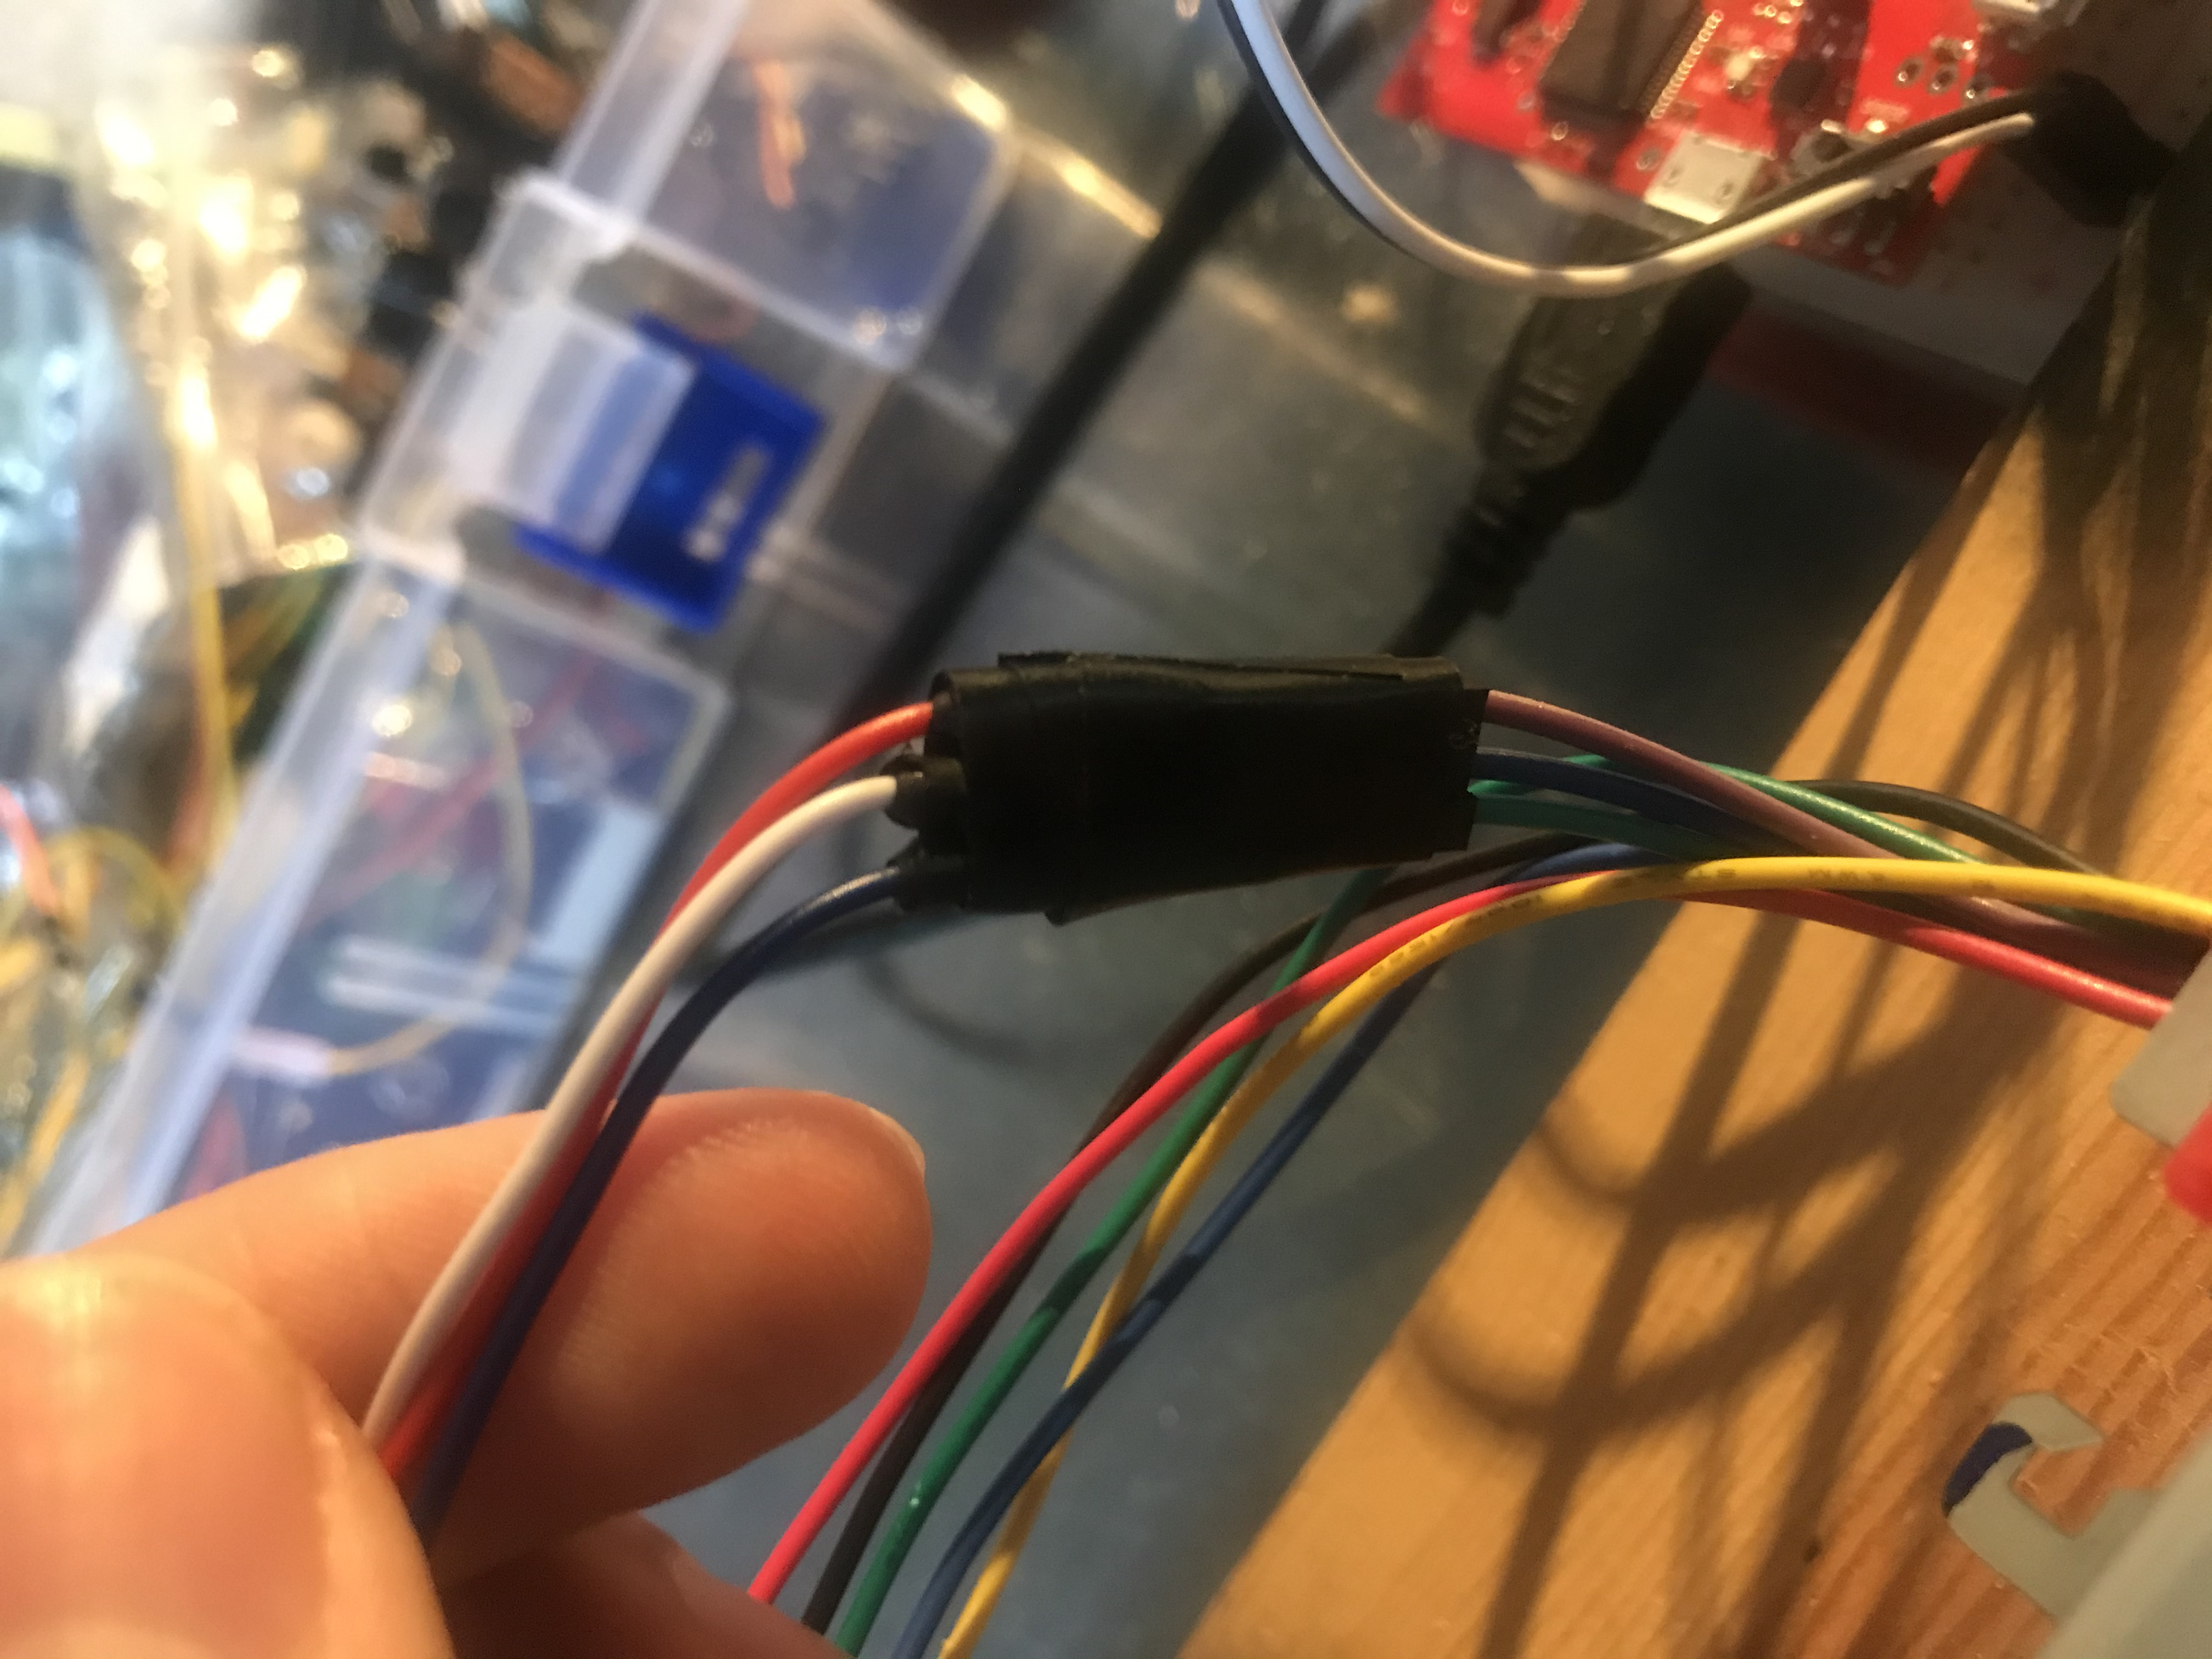
\includegraphics[width=1\linewidth]{figures/IMG_5968.jpg}
      \caption{Faulty Connection}
      \label{fig:conn}
    \end{subfigure}
    \begin{subfigure}{.4\textwidth}
      \centering
      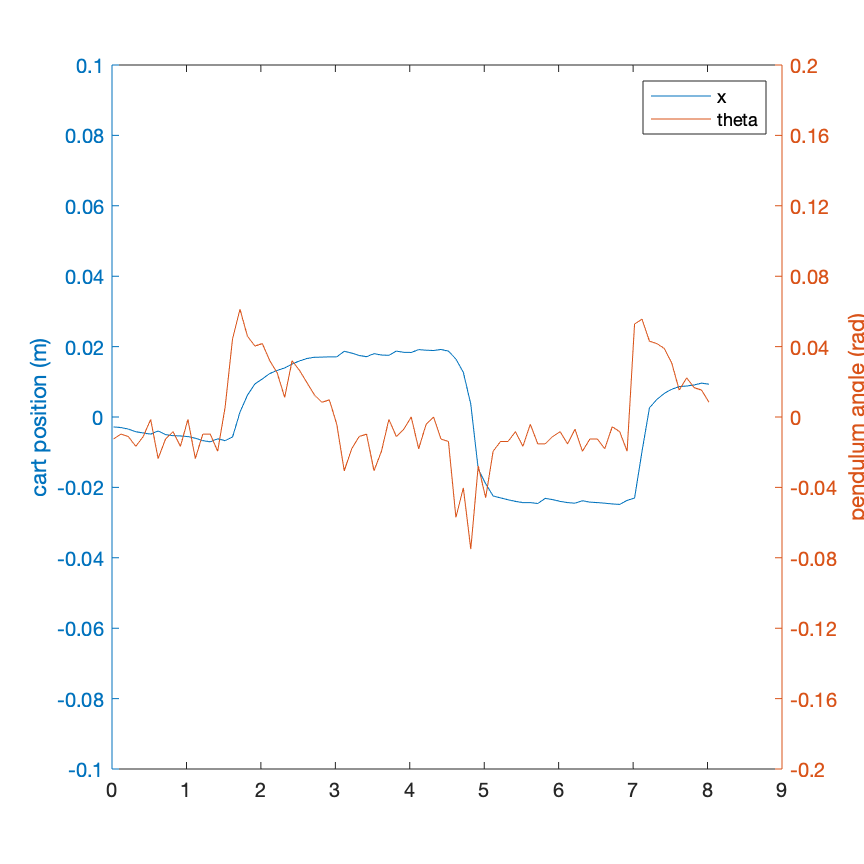
\includegraphics[width=1\linewidth]{figures/noise.png}
      \caption{Resulting Noise}
      \label{fig:noise}
    \end{subfigure}
    \caption{Faulty Connection Potentiometer Noise}
    \label{fig:senNoise}
\end{figure}

\subsubsection{Moving Average Filter for ADC Data}
When using an analog to digital converter, there is often a large amount of signal noise present, especially when using a cheap Arduino kit potentiometer. Thus, signal filtering is required. Rather than implementing an RC filter and delaying the signal with too large of a capacitor, we implemented a simple moving average filter. The following images display the before and after signal conditioning results.
\begin{figure}[H]
    \centering
    \begin{subfigure}{.32\textwidth}
      \centering
      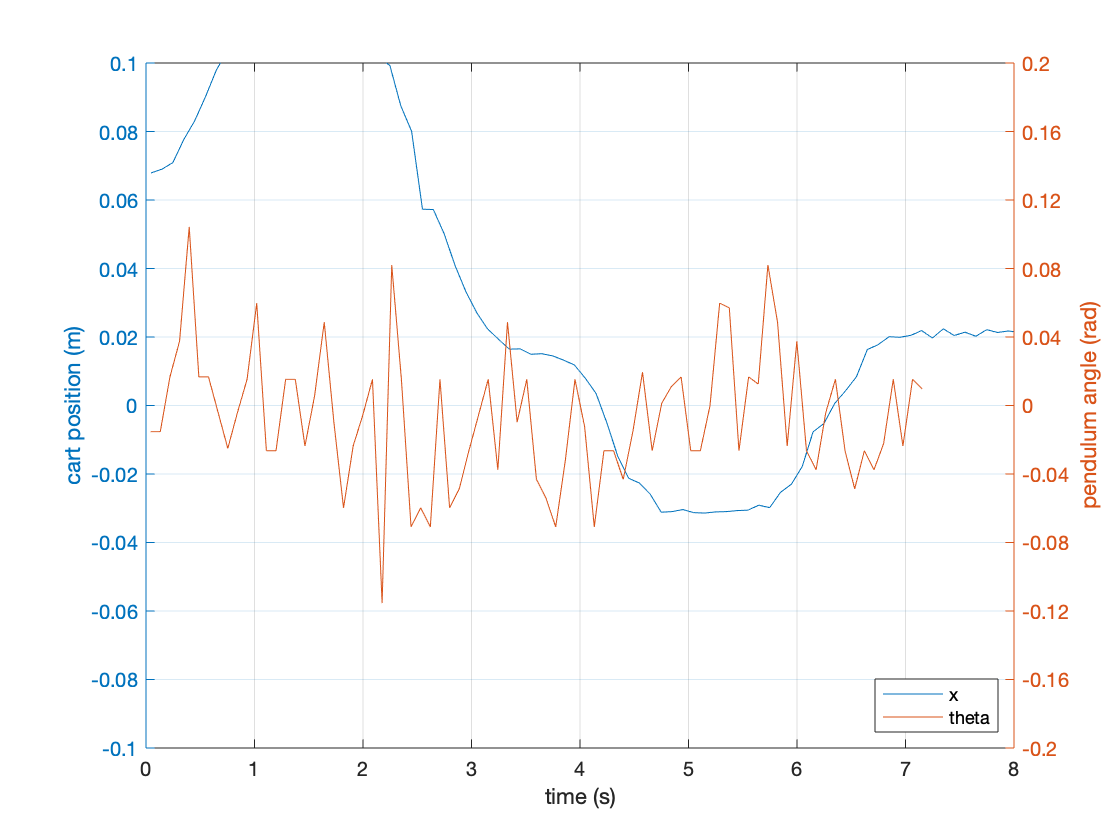
\includegraphics[width=1\linewidth]{figures/noAvg.png}
      \caption{No Filter}
    \end{subfigure}
    \begin{subfigure}{.32\textwidth}
      \centering
      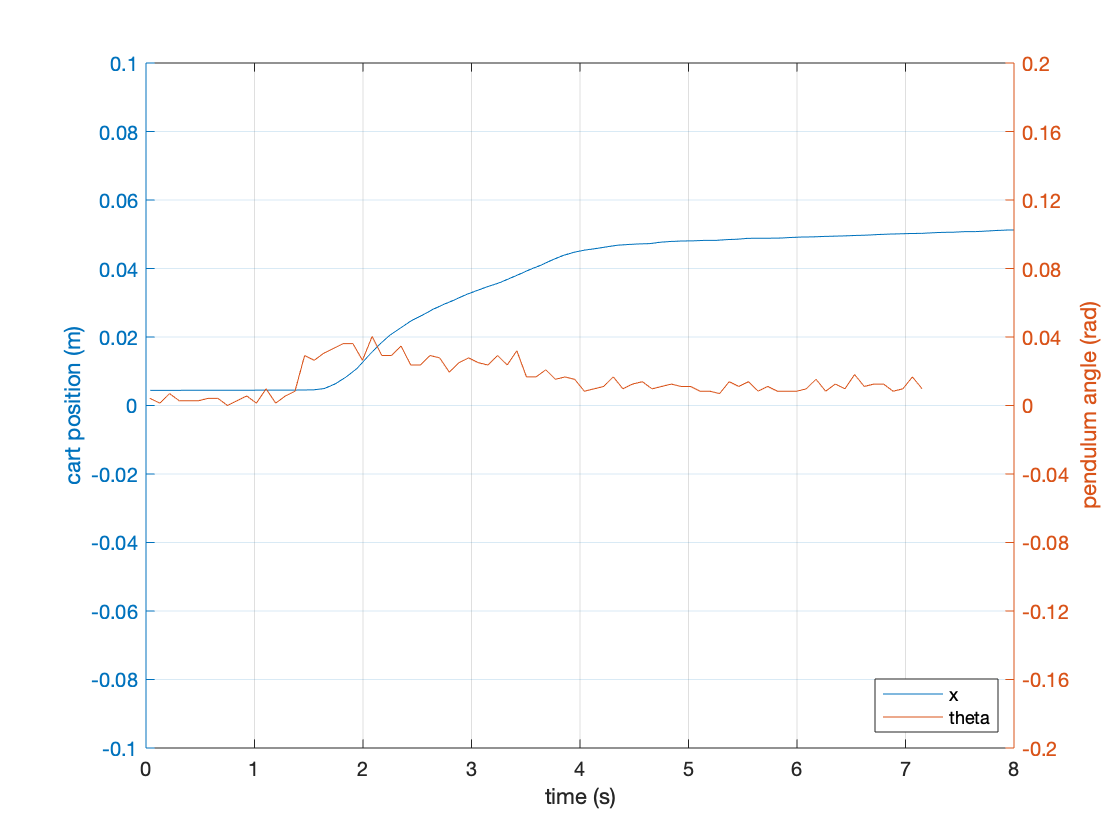
\includegraphics[width=1\linewidth]{figures/movAvg10.png}
      \caption{Moving Average, Length 10}
    \end{subfigure}
    \begin{subfigure}{.32\textwidth}
      \centering
      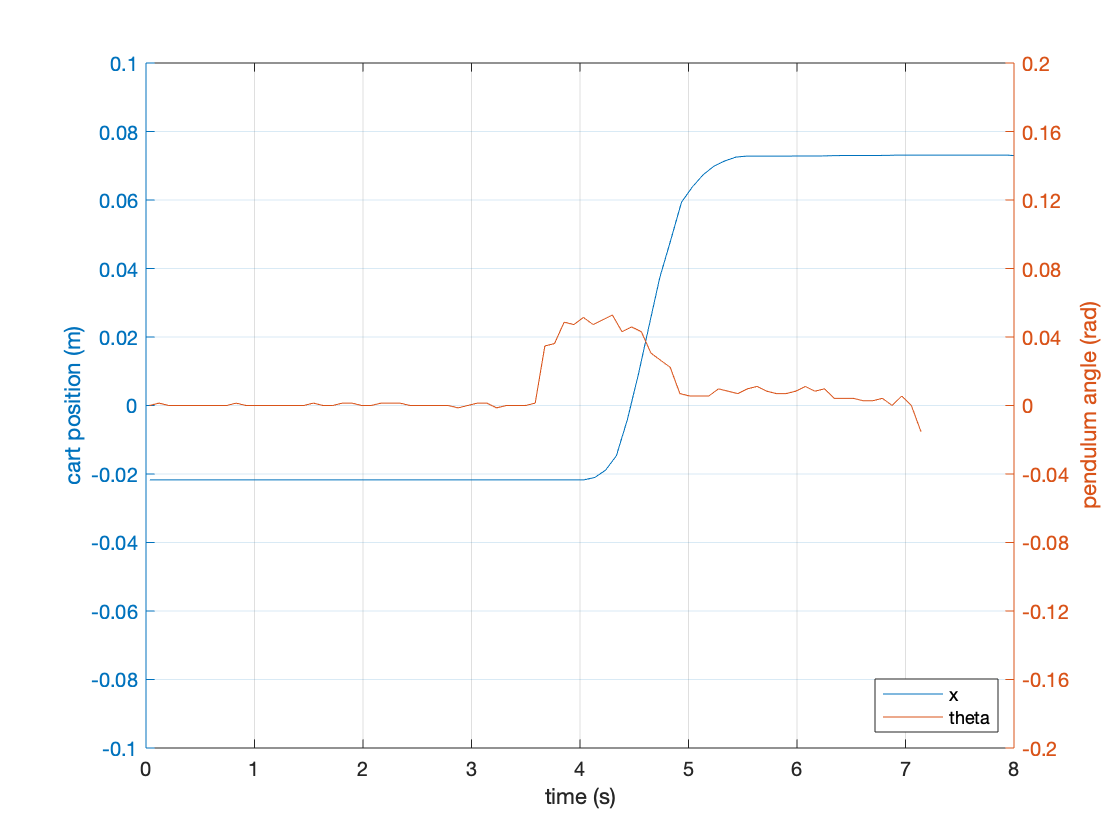
\includegraphics[width=1\linewidth]{figures/movAvg25.png}
      \caption{Moving Average, Length 25}
    \end{subfigure}
    \caption{ADC Signal Noise Moving Average Filtering}
    \label{fig:filter}
\end{figure}

\subsubsection{Quadrature Encoder Interface}
The Quadrature Encoder Interface (QEI) module provides an interface for which incremental encoders - such as the one used in this project- is able to obtain the mechanical position of the data \cite{qei}. Below is an image which illustrates the signals produced by a QEI (figure \ref{fig:qei}). These encoders are also known as optical encoders and characteristically have two signals which are out of phase (one leading and one lagging). Since the digital interrupt protocol for QEI outputs were not fast enough to increase or decrease the cart's position, the on board QEI peripheral was implemented. This was able to essentially read the cart's position separate from the main CPU. 

\begin{figure}[H]
    \centering
    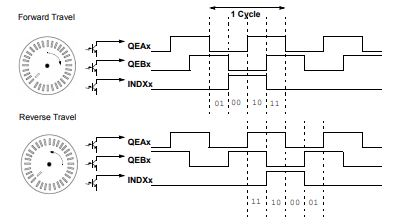
\includegraphics[width=.5\linewidth]{figures/qei.JPG}
    \caption{Quadrature Encoder Interface Signal}
    \label{fig:qei}
\end{figure}

\subsubsection{UART Data Transmission to MATLAB}
Rather than using Code Composer Studio's low quality graphical interface, that does not allow for recording of data, plot editing and more, UART communication was implemented on the board to enable plotting and analysis in MATLAB. Upon interrupt trigger, the board sends the current readings for $x$ and $\theta$, rather than constantly sending the data, even if no devices are listening. After a few lines of code, a loop allows MATLAB to poll these values from the board over a set period, convert them from hex to decimal, and plot. Code for the UART interrupt handler function can be seen in appendix \ref{uart}.


\section{Conclusions}
Overall, this system is completely feasible, controllable and observable. Within this control system design project we were able to provide thorough testing that was completed with all proposed components and ensured satisfactory working requirements to implement the state feedback controller. Issues that arose included the mechanical development and construction of the system requiring the complete deconstruction of the cart to be rebuilt in order create smoother movement. Furthermore, the optical encoder needed to be replaced as the old component salvaged from the printer was burnt out. Difficulties with protocol implementation included UART and PWM. UART was difficult to implement at first but was soon remedied after further research, and the PWM load cycle took a while to integrate during our experimentation but was able to run the motor successfully.
\\\\
Hours were spent tuning the system using MATLAB's \textbf{dlqr} function, which proved to produce a viable starting point \textit{K}. Finely tuning these gains enabled the system to respond quicker, and oscillate less. As for the implementation of the Luenberger observer state feedback controller, the tuning is nearing completion. Once this is completed, the system can be further tuned for faster response time, 0 steady state error and more. State space modelling in MATLAB has enabled the proper assessment of controllability and observability of the system, as well as tuning of the LQR controller.
\\\\
Overall, the project successfully implemented a state feedback controller. Of course if we had more time, an integrator would have been added to the LQR controller to eliminate steady state error, and the observer would have been completed - this will still be worked on by Ryan as a hobby project in the coming weeks of COVID-19 quarantine. All to date development can be seen on Github \cite{github}, on branch \textbf{master}. Gain tuning and Luenberger observer testing can be seen on branch \textbf{gain-tuning}, and will be merged once completed. Folder \textbf{matlab/} discusses system analysis, controllability and observability, as well as contains functions that were used for tuning the system. Folder \textbf{tiva/} contains all \textbf{C} code for the microcontroller board in Code Composer Studio.

\newpage
% ADD BIBLIOGRAPHY
\nocite{*}
\bibliographystyle{IEEE/IEEEtran}
\bibliography{IEEE/IEEEabrv,IEEE/biblio}

\newpage
\appendix
\section{Timeline}
It has been decided upon that the project duration will last approximately 1 month, to ensure completion of the working control system before the due date. The following timeline shows the approximate estimated dates for each major phase of the project. It should be noted that some tasks will be completed in parallel rather than in series, when possible. The remaining dates of April 1 - 10 will be used for tuning the controller with MATLAB and testing.\\

\begin{chronology}[5]{1}{30}{\textwidth}
\event{1}{Project Kick-off}
\event[1]{5}{Mechanical Setup}
\event[5]{8}{Wiring and Electronics}
\event[8]{11}{Integration Testing}
\event[11]{15}{Initialization (PWM, ADC, etc.)}
\event{15}{Individual Component Control Complete}
\event[15]{20}{BG Functions (Interrupts, ADC, etc.)}
\event{20}{System Implementation Complete}
\event[20]{25}{Control Model Development}
\event[25]{30}{Testing and Fine Tuning}
\event{30}{Project Deadline}
\end{chronology}
\textbf{Project Timeline for the Month of March, by Day}\\

\section{State Calculation in C}
\label{lqrctrl}
\begin{minted}[
frame=lines,
framesep=2mm,
baselinestretch=1.2,
fontsize=\footnotesize,
linenos
]{c}
void lqr(void){
    //xHat = pos posdot theta thetadot
    //need to estimate the derivative states, then apply exp avg filter
    float rPosDot = 0.05;
    float rThetaDot = 0.02;
    float rTheta = 0.15;

    xHat.X = (pos - ref.X)*scalePos;
    xHat.Y = (1-rPosDot)*posDotPrev + rPosDot*(xHat.X - posPrev)/dt;
    xHat.Z = (1-rTheta)*thetaPrev + rTheta*(4096.0 - read_ADC() - ref.Z)*scaleTheta;
    xHat.W = (1-rThetaDot)*thetaDotPrev + rThetaDot*(xHat.Z - thetaPrev)/dt;
    posPrev = xHat.X;
    posDotPrev = xHat.Y;
    thetaPrev = xHat.Z;
    thetaDotPrev = xHat.W;

}
\end{minted}


\section{Observer Function in C}
\label{obsverver}
\begin{minted}[
frame=lines,
framesep=2mm,
baselinestretch=1.2,
fontsize=\footnotesize,
linenos
]{c}
void obsv(void){
    y.X = (pos - ref.X)*scalePos;
    y.Y = (theta - ref.Z)*scaleTheta;

    yHat.X = HMM_DotVec4(C1, xHat);
    yHat.Y = HMM_DotVec4(C2, xHat);

    e = HMM_SubtractVec2(y, yHat);

    xHatDot.X = HMM_DotVec4(ABK1, xHat) + HMM_DotVec2(L1, e);
    xHatDot.Y = HMM_DotVec4(ABK2, xHat) + HMM_DotVec2(L2, e);
    xHatDot.Z = HMM_DotVec4(ABK3, xHat) + HMM_DotVec2(L3, e);
    xHatDot.W = HMM_DotVec4(ABK4, xHat) + HMM_DotVec2(L4, e);


    dt = stopTimer();

    xHatNext = HMM_AddVec4(xHat, HMM_MultiplyVec4f(xHatDot, dt));

    xHat = xHatNext;
    startTimer();

}
\end{minted}

\section{Observer Header in C}
\label{obsvh}
It should be noted that these actual gains were not implemented, only present at time of report development.
\begin{minted}[
frame=lines,
framesep=2mm,
baselinestretch=1.2,
fontsize=\footnotesize,
linenos
]{c}
//Gains for K, A-B*K, L from MATLAB
float k[4] = {-10,-10.7925,46.0882,7.94368};
float abk2[4] = {52.14475,55.60931,-239.0601,-41.42211};
float abk4[4] = {146.6096,156.7628,-651.391,-116.462};
float l1[2] = {430.0024,-162.9998};
float l2[2] = {5372.1669,-2736.4126};
float l3[2] = {-127.0637,177.8561};
float l4[2] = {3473.1059,110.9461};

\end{minted}

\section{UART Interrupt Handler in C}
\label{uart}
\begin{minted}[
frame=lines,
framesep=2mm,
baselinestretch=1.2,
fontsize=\footnotesize,
linenos
]{c}

void UARTIntHandler(void)
{
    uint32_t ui32Status;
    // Get the interrupt status.
    ui32Status = UARTIntStatus(UART0_BASE, true);
    //
    // Clear the asserted interrupts.
    //
    UARTIntClear(UART0_BASE, ui32Status);

    //UARTSend((uint8_t *)"nah\r\n", 5);
    //
    // Loop while there are characters in the receive FIFO.
    
    while(UARTCharsAvail(UART0_BASE))
    {
        // Read the next character from the UART and write it back to the UART.
        UARTCharPutNonBlocking(UART0_BASE, UARTCharGetNonBlocking(UART0_BASE));
    }
    send_u32(theta_target - theta);
    send_u32(pos);
}
\end{minted}



\end{document}
